\documentclass{article}
\usepackage[utf8]{inputenc}
\usepackage[margin=1.3in]{geometry}
\usepackage{amssymb,latexsym,amsmath,setspace,amsfonts,amssymb,amscd}
\setlength\parindent{0pt}
\setlength{\parskip}{\baselineskip}
\usepackage[colorlinks=true,allcolors=black]{hyperref}
\usepackage[english]{babel} 
\usepackage[normalem]{ulem}
%\documentclass{article}
\usepackage{graphicx}
\graphicspath{ {./images/} }
\usepackage{lastpage}
\usepackage{enumerate}
\usepackage{fancyhdr}
\usepackage{mathrsfs}
\usepackage[super]{nth}
\usepackage[dvipsnames]{xcolor}
\usepackage{tabto} 
\usepackage{amsthm}
\usepackage{multicol}
\usepackage{fancyhdr}
\usepackage{graphicx}
\graphicspath{ {./images/} }
\pagestyle{fancy}
\fancyhf{}
\lhead{MATH 3MB3 Project} %change the number 
\rhead{} % put your name and student number here
\cfoot{\thepage}
\setlength{\headheight}{15pt}


\begin{document}


\begin{center}
    \section*{Drugs in the Body}
    \subsection*{MATH 3MB3}
    \subsection*{April 21, 2022} 
    \section*{Junze Tan}
\end{center}

\section*{Background and Motivation}
Drugs are one of the most important subjects in any modern one’s life. This is especially true in the period of a global pandemic: after the outbreak of Covid-19, many countries, research institutes, and pharmaceutical companies have spent enormous effort on discovering, developing, and producing new vaccines and medications to help the global community to fight the pandemic. Just for the year 2021, 1467 Covid-19 related drugs are developed (Mikulic, March 2022) and used by more than 11,000,000,000 doses administered (Ritchie, March 2022), saving an uncountable number of lives.
 
Discovering and developing drugs is no easy job: not only should the researchers study the drug’s biochemical compositions to make sure it is effective and intoxic on the molecular/cell level (Reed, March 2022), but they have to also study the most effective way for drug administration: they need to find out when and how to administer the drugs so that its effects on the human body is the most desirable. The human body is a complicated system, for a drug to establish its desired therapeutic response, the concentration and duration of the drugs in the human body both play a vital part. For example, for some drugs to be effective, the concentration of the drugs in the blood has to exceed a certain level for a few hours; on the other hand, we need to carefully control the drug's concentration below a certain threshold and intervals because overdose on each drug may have adverse and irrecoverable effects on the human body (Reed, March 2022).
 
Predicting the effects of different drug administration is still an open question: there are many variables that jointly affect this process such as the drug itself, the delivery method, dosage, time intervals, human metabolic pathways, etc. There are many prior works that attempting to develop mathematical models to model this problem. Various numerical methods have been studied, including laplacian transformation and eigenvalue decomposition (Khanday, July 2016). Though the development of the mathematical model itself is purely theoretical, however, if verified with large amounts of experimental and clinical data, such a model can be very helpful in helping the researchers to design the most suitable drug administration methods empirically.
 
We are motivated by the great potential of modeling the effects of drug administration in developing new drugs. In this project, we aim to utilize our mathematical modeling knowledge to develop a few simple but effective models to study the effect of drug administration. In particular, we focus our research project on the effect of various delivery methods and metabolic pathways on a patient’s dosage over time.


\section*{Research Question Formulation}

Drugs metabolism involves different biological processes such as oxidation, reduction, hydration, etc. Regardless of what process is being used, the purpose is to ease the drugs excretion, which is the final step to clear the drugs from the human body. (Le, March 2022) Since the drug metabolism and excretion fully control the absorption and clearance of the drugs in the body, they are most studied by the researchers in assessing the best drug delivery methods and drugs dosage. Patients have different drug metabolism. This difference is a main contributor to interindividual variability in drug exposures and ultimately clinical response. Therefore understanding the processes that contribute to drug metabolism is of utmost importance to clinical pharmacologists. (Scott, 2022)

In this project, we aim to study the effect of various drug delivery methods and different metabolic pathways on the concentration of drugs in the human body. Our research question is below.

How does the body process a drug that is administrated through oral methods comparatively to intravenous methods?

Firstly, we aim to model the drug intake of the different drug delivery methods as the dosing rate $D(t)$, a function of the concentration of drugs as a function of time. We investigate various modes of drug delivery: oral vs intravenous, continuous vs discrete, different time intervals, and dosage. 

Secondly, we use a mathematical model to describe different metabolic pathways, be it a constant clearance model or a logistic model. We denote this metabolic pathways model by $p(A)$, the drug processing rate as a function of the current drug concentration $A(t)$.

Finally, we jointly consider how each combination of the drug delivery methods and the metabolic pathways affects the concentration of drugs in the human body. We denote this drug concentration by $dA/dt$, which is the rate of drug concentration change with respect to time. This model will be useful in predicting the effect of drugs on the human body, which in turn helps the researcher to design the most effective drug administration methods.

\section*{Base Model Construction}
Drugs can be administrated by various means, and each are designed to interact with the body in different ways. Typically the drug enters the blood stream, its effects take place, and the body metabolizes it and disposes of the drug. The rate of change of the drug in the body is dependent of the dose as well as the processing rate. These two parameters change depending on the type of drug as well as the person's age, gender, ethnicity, etc. All the factors are vital to consider when manufacturing a drug and needs to be tested over unbiased demographics to ensure it is a safe drug for all people. 

When creating a general model there are a number of assumptions made mathematically to make it as realistic as possible. 

Firstly, we assume the dosage is below the overdose rate but high enough that there will be an effect on the body. We are investigating how the drug will affect the body at an appropriate level. If it is above the overdose amount, the body will not behave as desired and lead to severe symptoms or even be fatal. For the Pfizer COVID vaccine, the overdose rate is 58 micrograms (EMA, 2021). For the purpose of this project we just want to analyze the drug as we intend it to function with an appropriate dosage.

Secondly, we assume that the body processes the drugs at an exponentially decaying rate, meaning it processes most of it at the beginning and as more drugs leave the body the body processes less of it. Realistically it only makes sense because the drug effects will gradually begin to increase and reach a peak before the body can return back to stability. This is why it is recommended that the patient is under supervision for 15 minutes after receiving the vaccine because more reactions will happen in this time period (EMA, 2021). 

Third, we assume the dosage rate is larger than the body's ability to process the drug, biologically if it was less the drugs will not have enough time to have an effect on the body.

Lastly, we assume that the processing rate and dosage rate are positive since we are looking at the instance where the drug enters the body and then is processed. These parameters would be negative if we were extracting a drug that the body produced because it was creating severe symptoms for the body. 

We will use a uni variate linear continuous deterministic model to describe the rate of change of the drug in the body. This is the best model because time in continuous and we will be able to calculate the amount of drugs in the body at any given time such as 2.45 or 3.999999 hours. We denote the state parameter, A(t) as the amount of drugs, measured in milligrams, in the body at time t hours. 

The model below describes how a drug is processed by the body where $D(t)$ is the dosing rate, measured in milligrams per hour and $P(A(t))$ is the processing rate, measured in units per hour. 

$$\frac{dA}{dt} = D(t) - P(A(t)) $$

D(t) is the dosing rate, measured in milligrams per hour. There are two cases of dosing we need to consider, first when there is dosing at rate r until time h, and then when the dosing stops after time h. 

\begin{equation}
  D(t) =
    \begin{cases}
      r & \text{if  $0 \leq t \leq h$}\\
      0 & \text{if $h< t$}
    \end{cases}       
\end{equation}

The processing rate, P(A) is described by cA(t) where c is the rate of how the body processes the drug measured in units per hour. It is dependent on A(t) so when there is a lot of drugs in the body the body will process more rather than when there is less in the body, the body will process less comparatively. 

$$P(A) = cA(t)$$

The parameters can be given values depending on the type of drug. For example, the Pfizer COVID-19 vaccine is administrated in 0.3mg doses approximately 21 days apart(EMA, 2021). The booster shot is given after a minimum of 5 months. So r would be 0.3 in this situation yet this model does not accurately represent the administration of vaccine since it is one dose at once, t= 0 and not a prolonged process to t = h. 

The processing rate, c, measured in units per hour, would be determined by the individual since each body reacts differently to each drug. Typically, as soon as the DNA or mRNA is inside the dendrite or tissue cells the cell use the instructions to create spike proteins, which usually takes less than 12 hours (CDC, 2021). So P(A) in this case would be less than 0.3 milligrams per 12 hours so an average of 0.025 milligram per hour. 

Since we can separate the dosing rate in two cases, we will split the equations separately, analyze them and then stitch them back together. Therefore we have the following model equations that describe the rate of change of drugs in the body.

The model equations are
\begin{align}
\frac{dA}{dt} &= D(t) - P(A) = r - cA(t) & 0 \leq t \leq h \\
\frac{dA}{dt} &= D(t) - P(A) = - cA(t) & t > h 
\end{align}

D(t),the dosing rate, where there is a consistent dose r measured in milligrams per hour from time t to h and after time h the dosing is stopped. When the drug is administrated by oral medication, such as tablets, pills, or liquids, these delivery methods of antigens needs to overcome multiple physicochemical and biological barriers in the gastrointestinal tract (National Library of Medicine, 2017). The drug must travel and encounter various biological and physicochemical mechanisms designed to prevent the entrance of foreign material to the body (National Library of Medicine, 2017). In order to overcome these obstacles, a larger dose is needed to instigate an immune response compared to other immunization methods (National Library of Medicine, 2017). For example, oxacillin, a drug used to treat infections caused by certain bacteria, has an oral dosage form of 500 milligrams to 1 gram every four to six hours and an injection dosage form of 250 milligrams to 1 gram every four to six hours for adults, teenagers, and children weighing more than 40 kilograms (Mayo Clinic, 2022). Therefore we will denote the dosing equation by s, between time $0 \leq t \leq h$ to describe this extra dosage needed where $r<s$

Oral Medications
\begin{equation}
  D(t) =
    \begin{cases}
      s & \text{if  $0 \leq t \leq h$}\\
      0 & \text{if $h< t$}
    \end{cases}       
\end{equation}

Intravenous Methods
\begin{equation}
  D(t) =
    \begin{cases}
      r & \text{if  $0 \leq t \leq h$}\\
      0 & \text{if $h< t$}
    \end{cases}       
\end{equation}


    
P(A) is the processing rate of the body measured in milligrams per hour and dependent on A(t) the amount of drugs in the body, measured in milligrams and c, measured in units per hour. The intravenous route is much more effective since the drug is immediately delivered to the bloodstream (Merck Manual, 2020), compared to an oral medication that needs to travel through the body before it reaches the desired location. The effect of the drug does not last as long and needs to be re-administered to maintain constant effect (Merck Manual, 2020). This means that the body processes the drug at a quicker rate than the oral medication and therefore the parameter c, needs to be modified to d, where c is smaller than d, to accurately describe the situation. 

Oral Medications

$$P(A) = cA(t)$$

Intravenous Methods

$$P(A) = dA(t)$$

For oral medications, many factors influenced the absorption rate such as age, gender, time of day, etc but it typically takes 30 minutes for the medication to dissolve (OCRC, 2016). For intravenous methods the body, the drug is absorbed instantly and will last in the body less than a day but the effects will occur more than a day (Next Health, 2022). The dosing period can take 45 minutes to an hour (Mobile IV Medics, 2022). 

Multiple Dosages

Multiple dosages are needed in order prolong effects and increase concentrations at a therapeutic level. Once the amount of drugs in the body reaches the therapeutic level, another dosage is given and will actually peak higher than the initial dose. Once it reaches an adequate level, the timing of the dosages and half life are important to calculate to maintain the steady state or else it will reach the toxic or level or therapeutic level. 

In order to have adequate concentration over a long period of time to fight an infection, multiple doses need to be administrated. For Penicillin, an antibiotic, a dose of 3-4 grams every 4-6 hours needs to be given because that is when the dosage will be therapeutic (Mayo Clinic) For oral medications such as Tylenol it is suggested to be taken every 6 hours. 

The model equations are the same except for the dosing. 

Oral Methods 

\begin{equation}
  D(t) =
    \begin{cases}
      s & \text{if  $t = Wn <h$ for $n\epsilon \mathbb{Z}$}\\
      0 & \text{if $h< t$}
    \end{cases}       
\end{equation}
where W represents the dosing interval time, for Tylenol in the example it would be W=6

Intravenous Methods
\begin{equation}
  D(t) =
    \begin{cases}
      r & \text{if  $t = Vn <h$ for $n\epsilon \mathbb{Z}$}\\
      0 & \text{if $h< t$}
    \end{cases}       
\end{equation}
where V represents the dosing interval time, for Penicillin in the example it would be V=6



This is what the model process would look like

\subsection*{Oral Method}

\begin{center}
    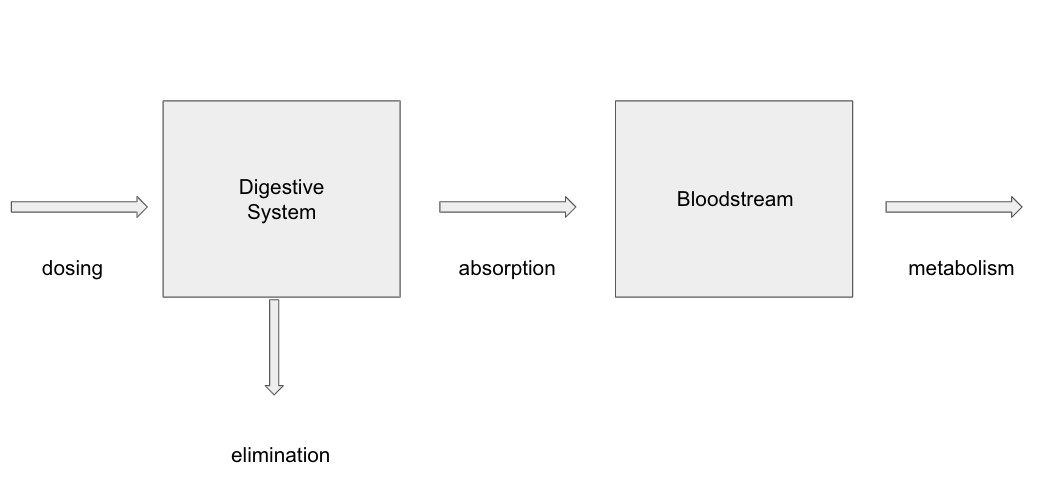
\includegraphics[scale = 0.4]{oral method graph .png}
\end{center}

\subsection*{Intravenous Method}

\begin{center}
    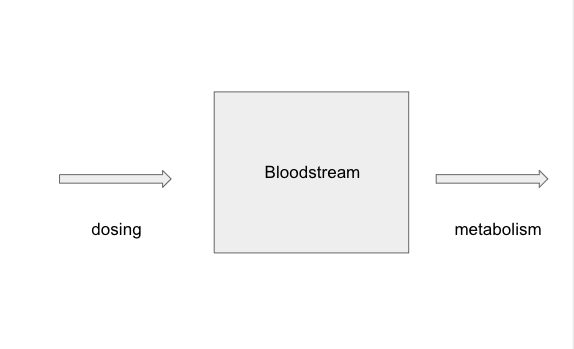
\includegraphics[scale = 0.5]{bloodstream.png}
\end{center}

\section*{Base Model Analysis}
This part will break down into parts to analyse the base model and simulate it to compare the difference in administrative methods. Generally, this analysis is using amoxicillin as a example, and discussing the difference between oral medication and intravenous method. Based on a research of University of Chile, the absorption constant of amoxicillin are 1.02 units/hour(Oral medication) and 1.16units/hour(intravenous method).(A.Arancibia et al, 1980) In our case, we are assuming the patient have Acute exacerbations of chronic bronchitis. Based on EMA, the proper dosage of this illness is 3g(3000mg) amoxicillin by oral medication(European Medicines Agency, 2022), or 750mg amoxicillin by intravenous method(European Medicines Agency, 2018). So, the above data will be used for the entire analysis section. For each sub-section, analysis will be discussed for both delivery methods. 
\subsection*{Equilibria}
Equilibria is significant in this model since it tells us the characterise long-term behavior. Not only the intravenous method and oral medications that are in our case, but also all drug absorption-kind model in our real world. 
Generally, the equilibria can be found when $\frac{dA}{dt} = 0$ as a ULCD model. That is $$0 = D(t) - cA(t)$$ where $P(A) = cA(t)$. Since D(t) is different by time t, when $t \in [0,h]$, $D(t) = r$. The equation will be $$0 = r - cA(t)$$ $$A(t) = \frac{r}{c}$$ for both r and c are constant and strictly positive. \\When $t > h$, $D(t) = 0$, the equilibria will $$0 = 0 - cA(t)$$ $$A(t) = 0$$ Which is also make sense. As we stop dosing drugs, the body has absorbed all drugs remaining after time h. The amount of drugs in body is 0.\\
If we break down it into 2 cases, the equiliria will be:
\begin{itemize}
    \item Oral medication: based on previous model construction, we are assuming the drug is dosed instantaneously, which means the dosage equal to 3000mg at time $t = 0$. Then, the fixed point will be $A(t) = \frac{3000}{1.02}$. That is $A(0)  \approx 29411.18$. When the time $t>0$, there is no more dosage. So, the equilibria will be $A(t) = 0$.\\
    \item Intravenous method: According to the European Medicines Agency, the intravenous dosing of amoxicillin usually takes 30-60 minutes. We will take 60min(1 hour) as our assuming dosing period. So, when time $t \in [0,1]$, $D(t) = 750$. The equilibria will be $A(t) = \frac{750}{1.16}$, that is $A(t) \approx 646.55$ mg. Similarly, the equilibria after dosage ($t > 1$), will be $A(t) = 0$.
\end{itemize}

The equilibrium is an important aspect to study because it tells researchers when to expect the peak of drugs in the body, this is when the processing rate is larger than the dosing rate and the body will begin to dispose the drug and the effects of the drug will begin to wear off. Since oral medications and intravenous methods have different dosing and processing rate they are difficult to compare. Yet the key difference is that for oral medications the equilibrium is when t = 0 and for intravenous methods it occurs between $0<t<h$. This means that the body begins processing oral medications immediately because it is a one time dose, rather than for intravenous methods the equilibrium occurs later so the body needs a whole hour before the body can begin processing. The findings are vital to explore to know when to expect how the body behaves to the drug and when it is safe to begin dosing again to not risk overdosing and ensuring maximum effectiveness will occur again safely. If the dosing begins too soon, before the body has a chance to full dispose and recover from the drug, the next dose might lead to overdose, undesired behaviour or not be as efficient. Now that we know the equilibrium occurs when the amount of body in the drugs is equal to the ratio of the dosing rate and processing rate, we can derive conclusions of what the processing rate is and understand what factors affect this model. 

\subsection*{Stability}
Understanding the stability of the equilibrium is crucial to comprehend when creating a drug. The stability will tell us the behaviour of the drug and how we can predict it's future fluctuations.\\

\subsubsection*{Oral Medication}
In this case, we can sketch both $t = 0$ and $t > 0$ in one graph below. \\

\begin{center}

  
      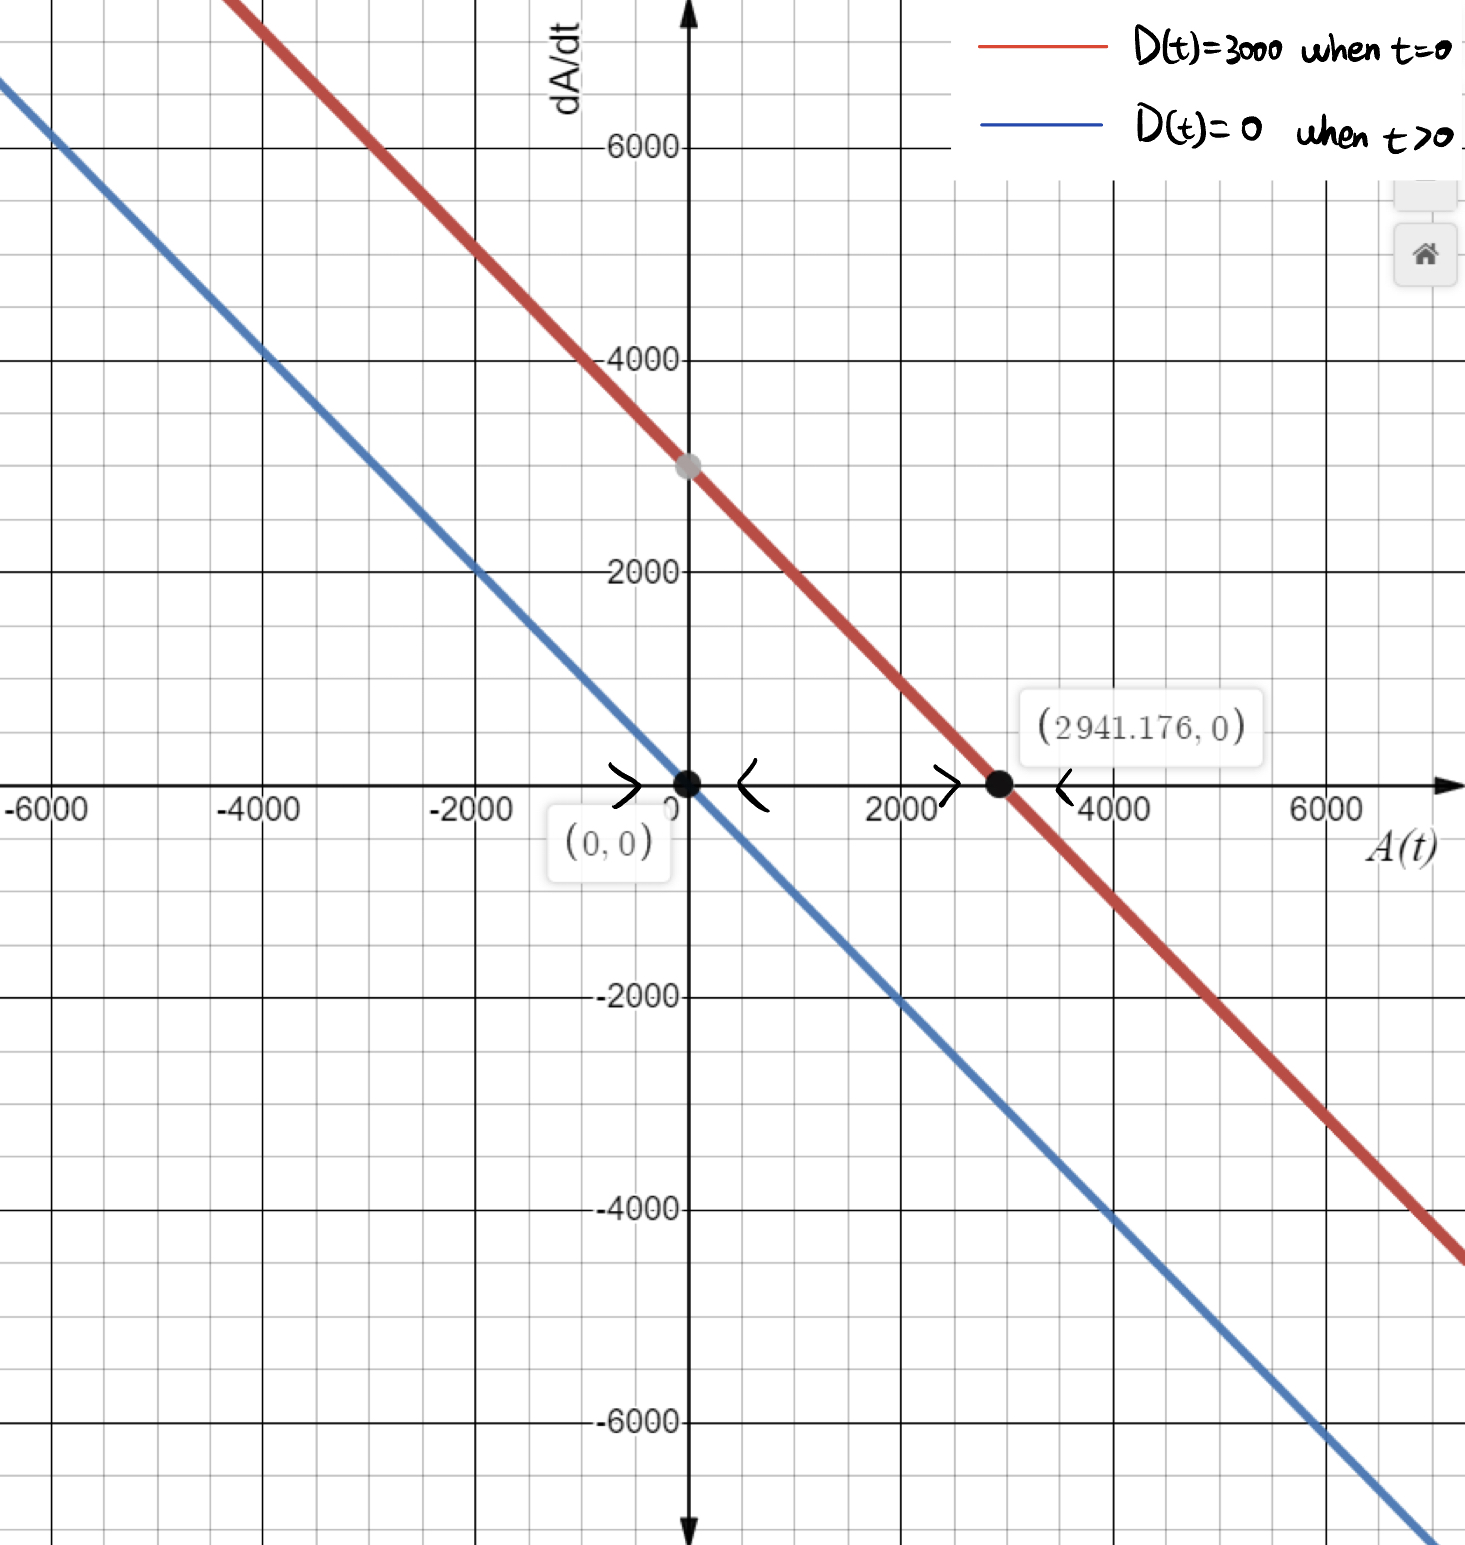
\includegraphics[scale = 0.15]{oralStab.jpg}


\end{center}
        
        



Stability can be determined by the value of $\frac{dA}{dt}$. Firstly, we can focus on the two sides of $A(t) = 29411.18$ that is the fixed point when $t = 0$. When $A(t) < 29411.18$, $\frac{dA}{dt} > 0$. When $A(t) > 29411.18$, $\frac{dA}{dt} < 0$. So, it towards to the fixed point from each sides, which means it is stable. \\
Similarly, when $t>0$, it is also stable since both sides moving towards to the fixed points.
\subsubsection*{Intravenous Method}
For analysing the stability of intravenous method, we can also use the graphical approach. \\
\begin{center}
    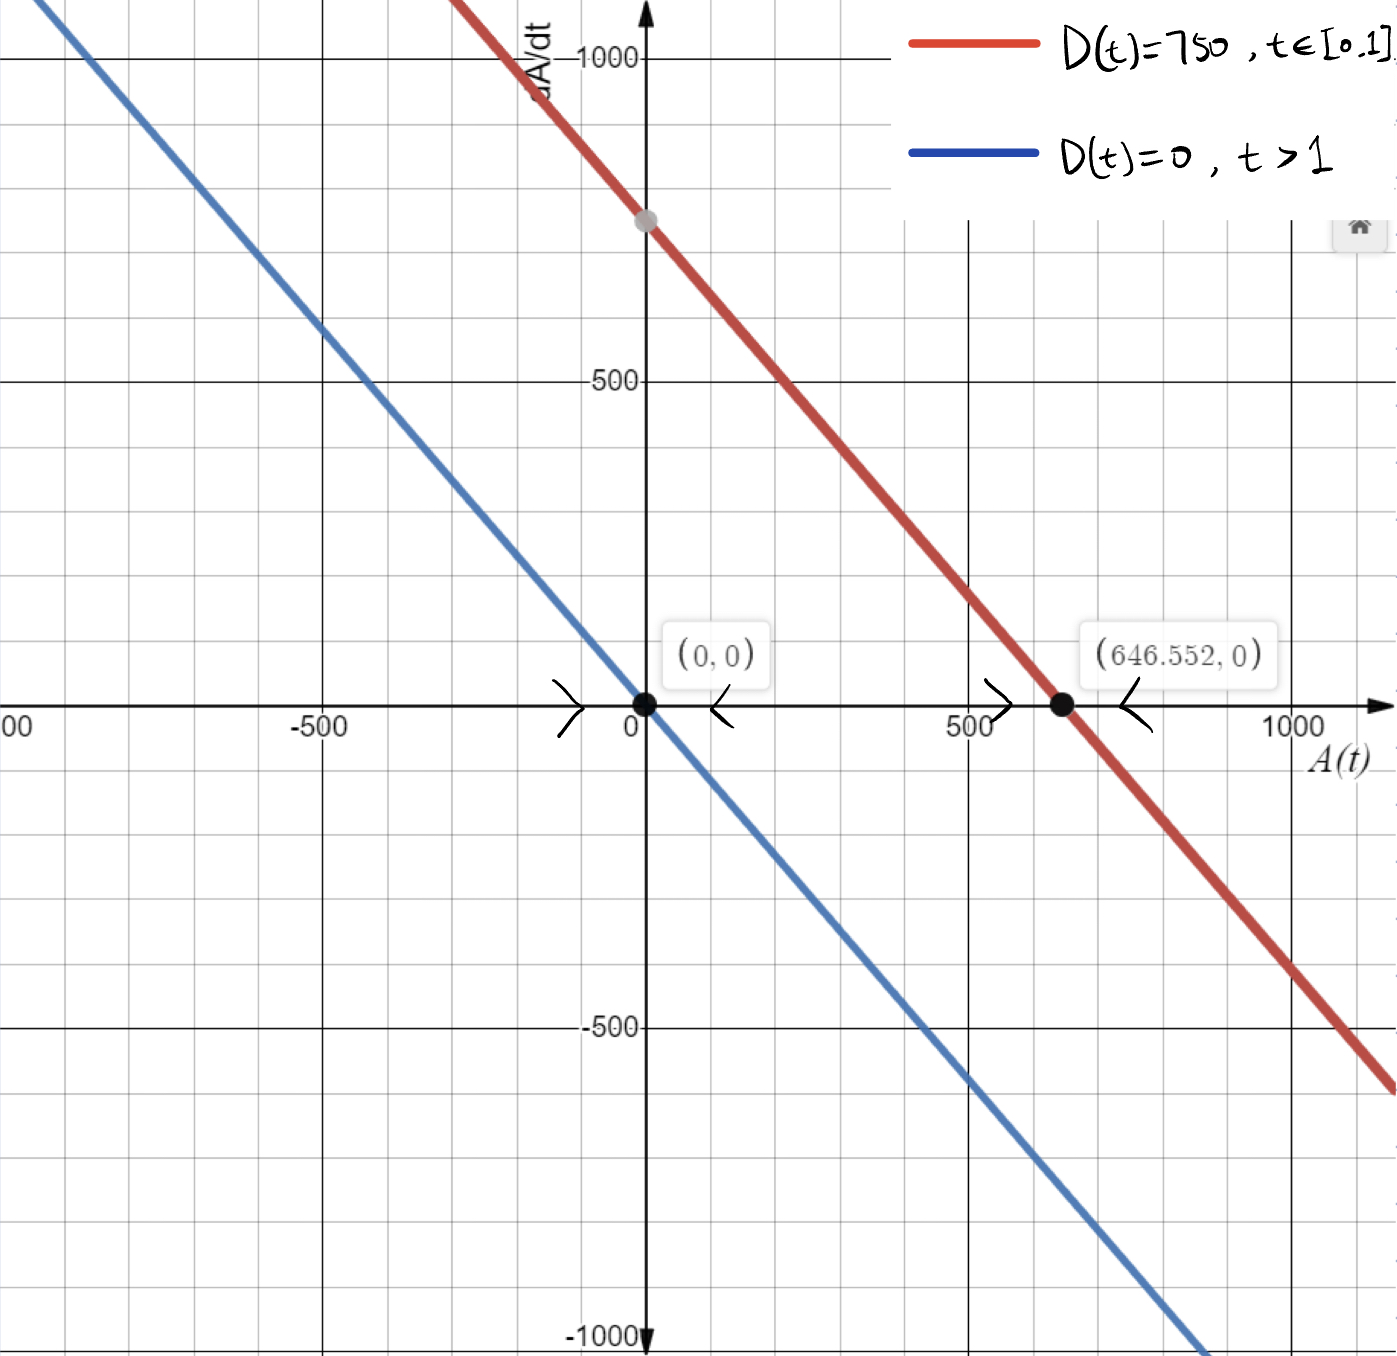
\includegraphics[scale = 0.15]{IntravStab.jpg}
\end{center}


    
By the graph, we can see both $t\in [0,1]$ and $t>1$ are stable at each fixed points. Since both function have $\frac{dA}{dt}$ towards to the fixed point.\\

Although we might not have a negative clearance rate in our real life. Mathematically, we can discuss the stability when we have a negative clearance rate which means there are some drugs is produced by human body. In this scenario, we are assuming human body is producing some drugs at a rate of 1.5 units/hour(c = -1.5). The graph will be as below\\
\begin{center}
    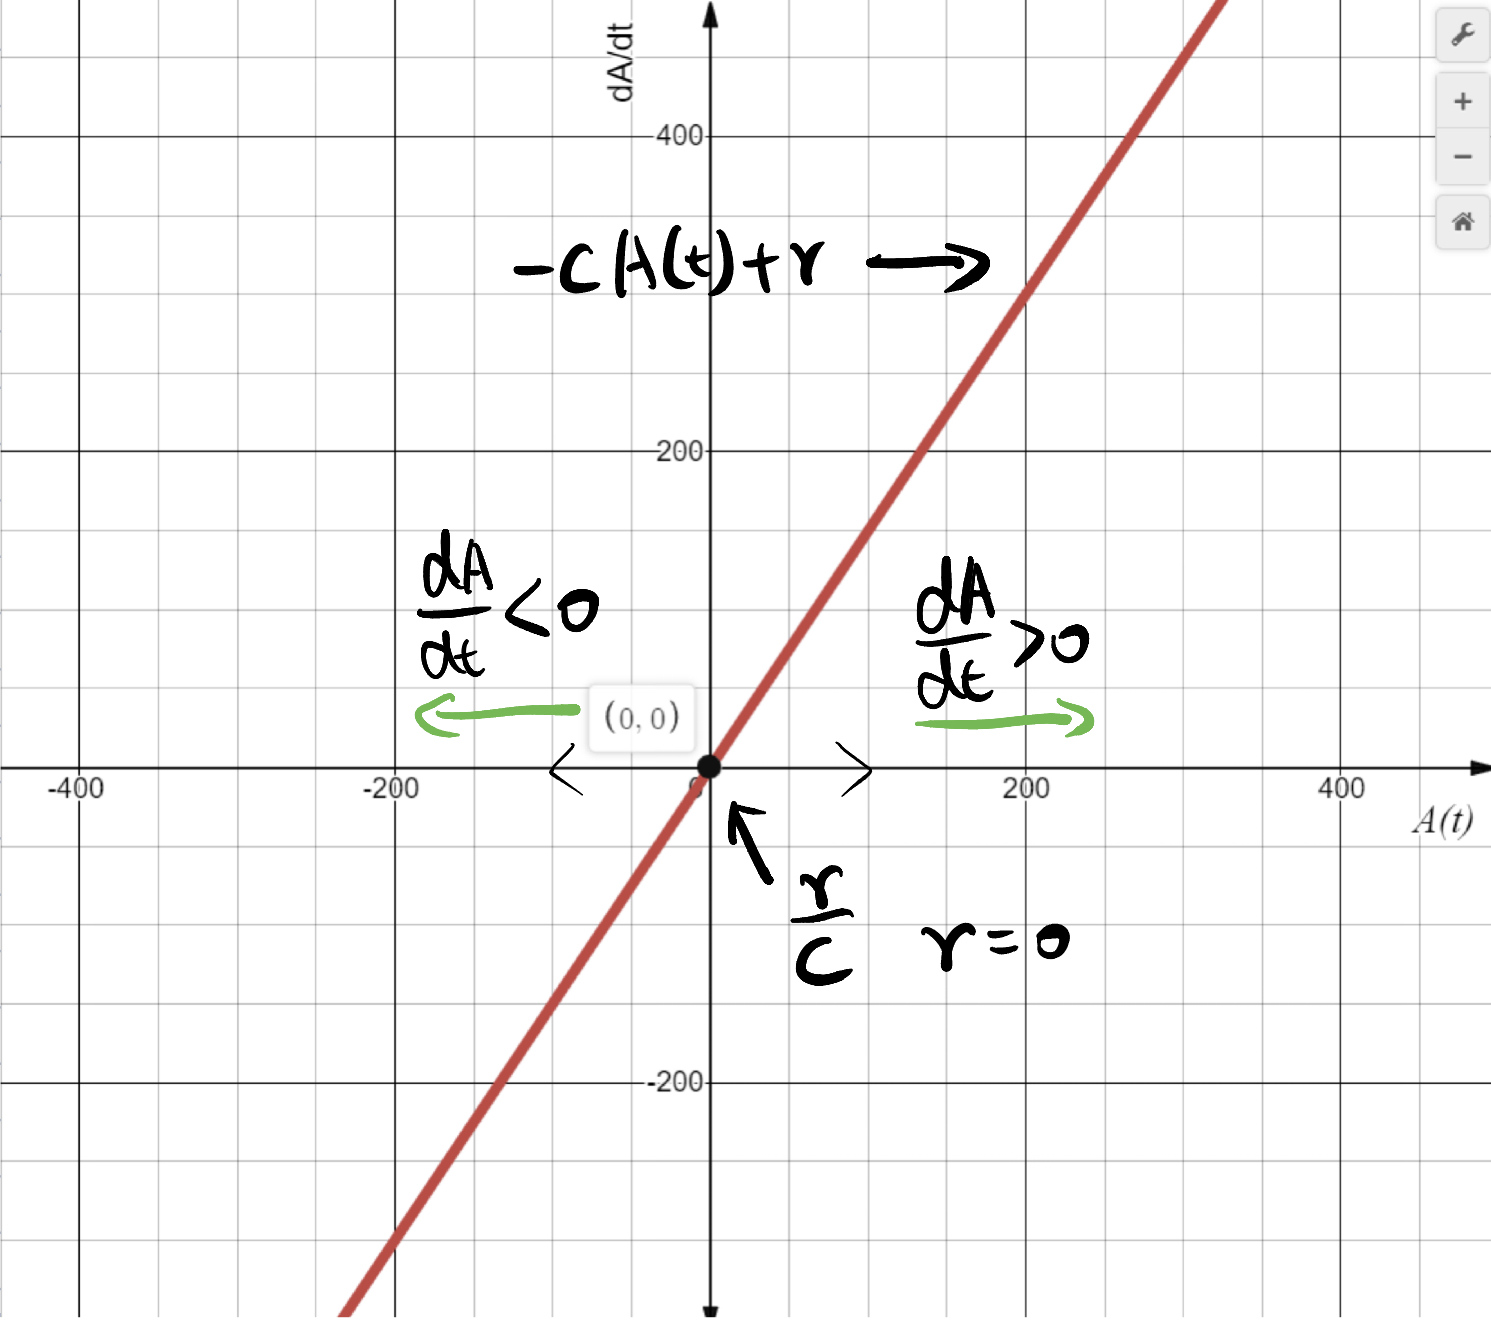
\includegraphics[scale = 0.15]{negtiveStab.jpg}
\end{center}
So, we can find that it is unstable when we have a negative clearance rate at the fixed point. The value of $\frac{dA}{dt} < 0$ when $A(t) < 0$, and  $\frac{dA}{dt} > 0$ when $A(t) > 0$. That is pointing outward from the fixed point. Hence, it is unstable. In this case, our body is producing a drug that the body is trying to get rid of. For example, Creatinine, a waste product made by muscles which is part of everyday activities, is an ideal way to measure kidney function because if there is a problem in the kidney, the Creatinine will not appear in the urine and will be built up in the blood. (Mayo Clinic, 2021)

Since the solution is unstable in this case, we know that the drug will increase exponentially so treating the disease right away is vital for the body to survive. In a short period of time, if the kidney can not process the Creatinine, this will indicate that there is kidney malfunction which can be fatal if not treated. 

When the solution is stable we know that small minor fluctuations will not be successful in deteriorating our desired results, unlike in the negative clearance rate case when the equilibrium is unstable, small perturbations will eventually grow at a much quicker rate than our parameters and disturb the process.

Since the derivatives are moving towards the equilibrium we are confident to predict that the peak occurs at $A(t) = \frac{r}{c}$
We know exactly what to predict after the dose is administrated at every given point and be able to conclude when the drugs should not be detected in the body giving us an goal and therefore an indication on if the drug is being processed safely. 



\subsection*{Analytical solution}
Analytical solution can helps us to understand the entire model from the parameters. Once we have the analytical solution, we can know how each variables work in the A(t) function. Basically, the way of find analytical solution for both methods are the same. The analytical solution can be found by solving $\frac{dA}{dt} = D(t) - cA(t)$. The general form can be written as\\

When $t \in [0,h]$, it will be 
$$
\frac{dA}{dt} = r - cA(t)
$$
$$
\frac{1}{-cA(t)+r}dA = dt
$$
Let $u = -cA(t) + r$. Then $du = -c*dA$,$dA = \frac{1}{-c}du$.
$$
\frac{1}{u}(\frac{1}{-c})du = dt
$$
Integrate both sides.
$$
\int_{u(A(0))}^{u(A(t))} \frac{1}{u}(\frac{1}{-c}) du = \int_{0}^{t} dt
$$
$$
\frac{\ln u}{-c} = t + k
$$
where k is some constant caused by integration.\\
Then, we can substitute $u = r- cA(t)$ back in to the equation.
$$
ln(r-cA(t)) = -ct+k
$$
take away the ln for both sides,
$$
r-cA(t) = e^{-ct+k}
$$
$$
-cA(t)= e^{-ct+k}-r
$$
$$
$$
The analytical solution of this model when $t \in [0,h]$ will be
$$
A(t) = \frac{-ke^{-ct}+r}{c}
$$
When $t > h$, the analytical solution will be
$$
\frac{1}{-cA(t)}dA = dt
$$
integrate both sides,
$$
\int \frac{1}{-cA(t)} dA = \int dt
$$
$$
\frac{1}{-c} \ln{A(t)} = t + k
$$
where k is come constant caused by integration.\\
$$
\ln{A(t)} = -ct+k
$$
So, the analytical solution when $t > h$ is
$$
A(t) = ke^{-ct}
$$
Then, we discuss the solution separately by different methods.\\
For oral medication, since we are assuming the dosing is instantaneously, then the analytical solution at $t = 0$ is $A(0) = 3000$. After time 0, the amount of amoxicillin in body starts exponentially decaying in form of $A(t) = ke^{-1.02t}$.\\
On the other hand, the analytical solution for intravenous method will be $A(t) = \frac{-ke^{-1.16t}+750}{1.16}$ for all $t \in [0,1]$. After one hour, the analytical solution will be $A(t) = ke^{-1.16t}$\\
So far, we have got the analytical solution for both cases. We can use it for our real world simulation.
\subsection*{Simulation with real-world context}
After all basic analysis, we can combine those components with real-world context so that we can know more about different delivery method will varies the body absorption. By using Python, we can visualised the models of each delivery method. 
\subsubsection*{Oral medication}
Firstly, we are using the same data from above by EMA. Therefore, the dosage r at time 0 is 3000 mg, and the body have a clearance rate of 1.02 units/hour. Since the oral medication is dosed instantaneously, we have a $x0 = 3000$ at $t = 0$. \\
\begin{center}
    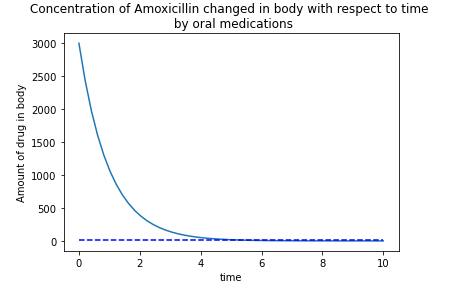
\includegraphics[scale = 0.7]{simuOral.png}
\end{center}
From the graph, we can see the amount of amoxicillin in body is 3000mg at the begining. As a exponential decay graph, the concentration of amoxicillin decreases dramatically. We know the analytical solution of oral medication is $A(t) = ke^{-1.02t}$ after time $t = 0$. Mathematically, the exponential decay graph can not reach 0 whatever how long the time passed since we are dealing with e to the power of variable. So here we are using a parameter undetectable amount $und = 10$ as the amount of drugs that can not detected by current technology. Briefly, the concentration of amoxicillin in body is under the undetectable amount after 4 hours. So, the oral medication of 3000 mg amoxicillin can be entirely processed by adult body within 4 hours.\\

\subsubsection*{Intravenous method}
According to EMC, when dosing amoxicillin by intravenous method, the adult clearance rate is 1.16 units per hour. So, here we have $c = 1.16$. With 750 mg amoxicillin dosage will be done in one hour. Then, $D(t) = 750$mg per hour with a dosing period 1 hour, that is $t\in [0,1]$. Combining with those factors, we obtain the graph as of below.\\

\begin{center}
    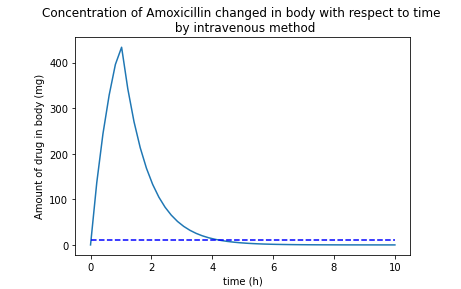
\includegraphics[scale = 0.7]{simuIntra.png}
\end{center}
As shown in figure, we have no amoxicillin in body at time 0. As we start dosing, the concentration of amoxicillin in body also start increasing. Since the dosing rate is greater than the processing rate. Any time $t\in [0,1]$, the value of $\frac{dA}{dt}$ is greater than 0. As $t > 1$, the dosing stop, we can find a dramatic exponential decay. Finally, the concentration of amoxicillin is processed as a undetectable amount $und = 10$mg after approximately 4 hours. \\

Although both delivery method takes about 4 hours to process all amoxicillin. The drugs only works when tissue concentrations reached for sufficient time.(Jennifer Le, 2020) From the figure, we can see that intravenous method have a relative stable high-concentration period before all amoxicillin has been processed. In other words, the intravenous method can provide a batter treatment performance than oral medication. A journal from Pharmacol Pharmacother states that, "Bioavailability of IV medications is always higher than that of their oral counterpart."(J Pharmacol Pharmacother, 2014) That is also what we found after analysis. Hence, theoretically, intravenous method helps patients get relief from symptoms earlier than oral medications. \\

This answers our research question of the differences of intravenous methods and oral methods. Yet, for some drugs pills are a better way since they are easily administrated, not as susceptible to infections, and easily accessed. Scientist choosing the method needs to determine what their priorities are and what resources are available. If they believe high concentration is most important and they have trained professionals to administrate a shot, then the intravenous method would be preferred, like a vaccine. Yet if accessibility is more important then a pill for antibiotics would be a better method. There is not one method that is better than the other, rather which method best serves the people with available resources. 

\section*{Proposed Model extension}
For the Proposed Model extension, this is the expansions of the base model. In this project we are going to discuss two extension models.
\subsection*{Logistic model}
First is called the logistic model. Instead of $P(A)=cA$, we have $P(A) = cA(1-A/K)$ where c has the same definition as the clearance rate and K is a new logistic parameter. Here we need to think about what could k be. From the formula we can find k also can effect the speed of the drug to be absorbed. Let's assume k as how many times the blood can flow a round per hour. From the research we can assume k = 60 since the blood travels the whole body may take about 1 minute. This is the average count because the blood will go through the different size of blood vessel, so the speed and time is different.\\

As before, the dosing rate is still the same which is:
\begin{equation}
  D(t) =
    \begin{cases}
      r & \text{if  $0 \leq t \leq h$}\\
      0 & \text{if $h< t$}
    \end{cases}       
\end{equation}

But the clearance rate will change to 
\begin{equation}
  P(A) = cA(1-\frac{A}{K})
\end{equation}

Now, the whole logistic model equation will be:
\begin{equation}
  \frac{dA}{dt} =
    \begin{cases}
      r- cA(1-\frac{A}{K}) & \text{if  $0 \leq t \leq h$}\\
      - cA(1-\frac{A}{K}) & \text{if $t > h$}
    \end{cases}       
\end{equation}

\section*{Logistic Model Analysis}

The base model can not accurately describe the drug's behaviour for every person. Due to their genetics and lifestyle habits, they will have different processing rates which will in turn effect the efficiency and effects of the drug. Using a logistic parameter to describe these situations can help us understand what we can predict when creating a drug,


\subsection*{Equilibria}
Equilibria is a point could keep a balance on both side. In this project,the equilibria is the drug in the body can be a stable system which all influences are balanced or canceled. To solve the equilibria of this logistic model we can let $\frac{dA}{dt}=0$ which means let $r-cA(1-\frac{A}{K})=0$ and $-cA(1-\frac{A}{K})=0$.

When $r-cA(1-\frac{A}{K})=0$\\
$$
c(-\frac{A^2}{k}+A)=r
$$
$$
A^2-Ak=-\frac{r}{c}k
$$
$$
A^2-Ak+\frac{1}{4}k^2=-\frac{r}{c}k+\frac{1}{4}k^2
$$
$$
(A-\frac{1}{2}k)^2=-\frac{r}{c}k+\frac{1}{4}k^2
$$
we can get $A(t)=\frac{1}{2}k+\sqrt{-\frac{r}{c}k+\frac{1}{4}k^2}$ and $A(t)=\frac{1}{2}k-\sqrt{-\frac{r}{c}k+\frac{1}{4}k^2}$ 

When $-cA(1-\frac{A}{k})=0$\\
$$
-cA=0
$$
$$
A=0
$$
$$
1-\frac{A}{k}=0
$$
$$
A=k
$$
we can get $A(t) = 0$ and $A(t) = k$ 

\subsection*{Stability}
Stability in this project means the ability to avoid the effect from other influence factors. From the lecture, we learned how to determine the stability of logistic model. It's different from the base model. We need to first find out the derivative of $\frac{dA}{dt}$.\\
\\
For $0 \leq t \leq h$:
$$
\frac{dA}{dt}= r - cA(1-\frac{A}{k}) = f(A)
$$
$$
f(A) = r - cA + \frac{c}{k}A^2
$$
$$
f'(A) = - c + \frac{2c}{k}A
$$
$$
When A(t)=\frac{1}{2}k+\sqrt{-\frac{r}{c}k+\frac{1}{4}k^2}
$$
$$
f'(A) = \sqrt{-\frac{r}{c}k+\frac{1}{4}k^2}
$$
This point is unstable, that means the drugs peak in the body at this point. Similar to the base model, the body will peak between time 0 and h, after the dosing stops. 

When $A(t)=\frac{1}{2}k+\sqrt{-\frac{r}{c}k+\frac{1}{4}k^2}$:

$$
f'(A) = -\sqrt{-\frac{r}{c}k+\frac{1}{4}k^2}
$$
Which is stable. 

For $t > h$:
$$
\frac{dA}{dt}= - cA(1-\frac{A}{k}) = f(A)
$$
$$
f(A) = - cA + \frac{c}{k}A^2
$$
$$
f'(A) = - c + \frac{2c}{k}A
$$
When $A(t)= 0$
$$
f'(A) = -c < 0 
$$
Which is stable. Then this point is a minimum which makes sense since there is zero dosing and will exponentially grow as the dosing begins. 

When $A(t)= k$:

$$
f'(A) = c > 0
$$
Which is unstable.

\begin{center}
    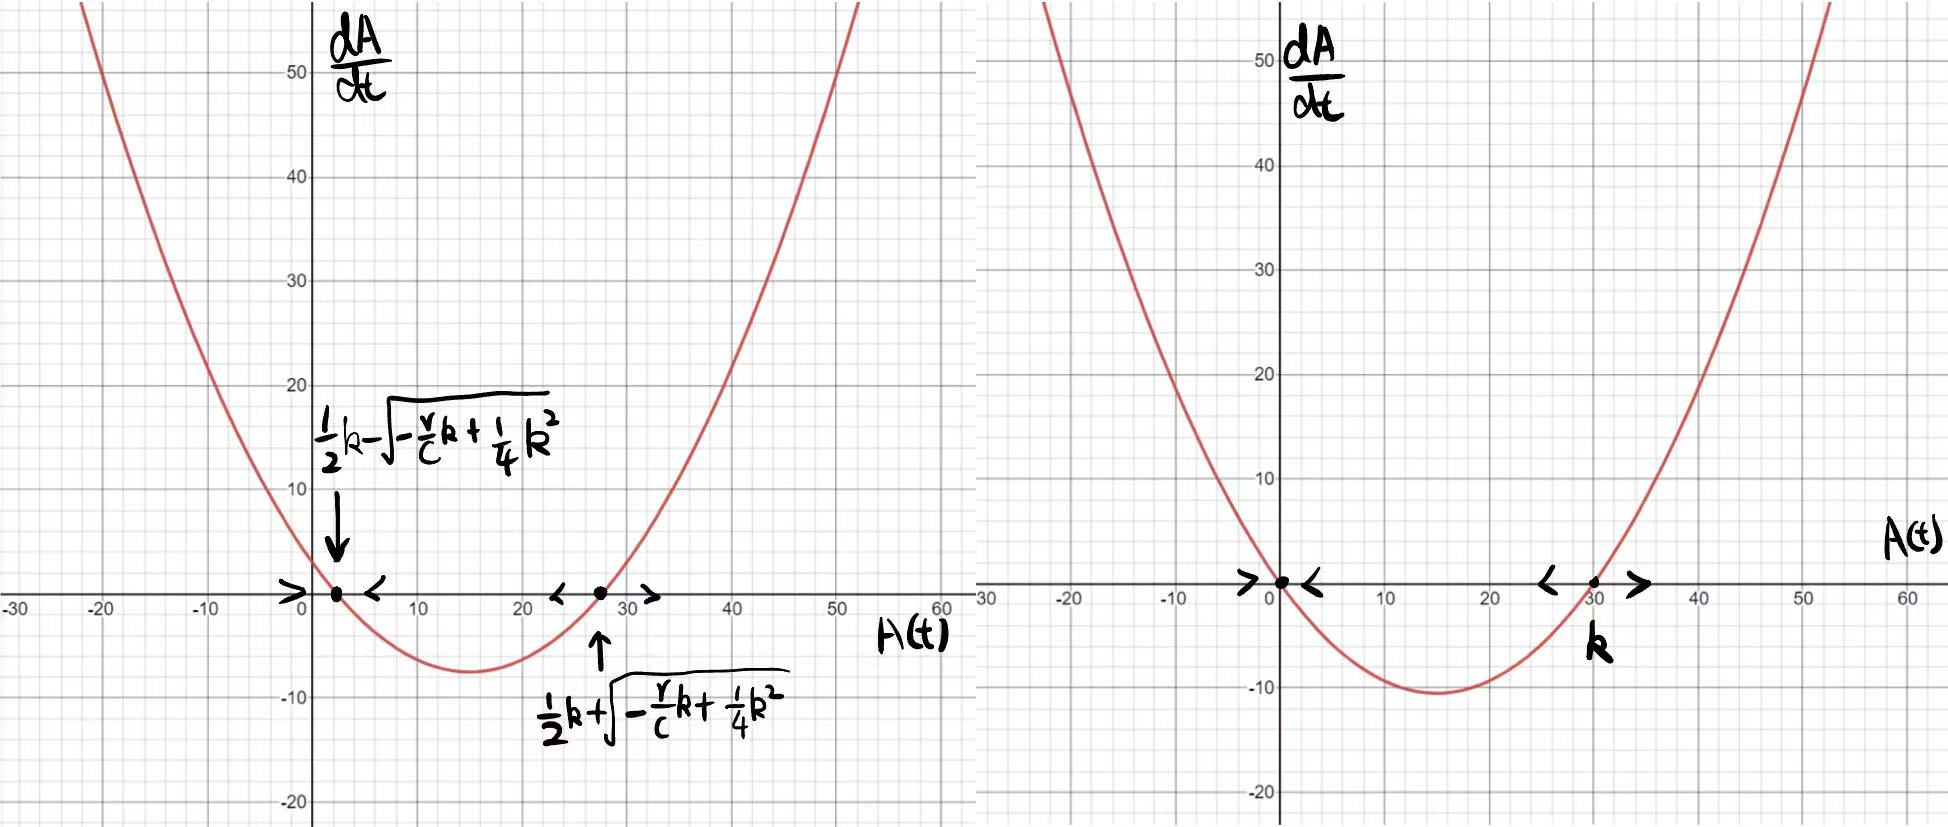
\includegraphics[scale = 0.2]{stability_of_logistic.jpg}
\end{center}

The left one is when $0 \leq t \leq h$. We can see that two arrows on the both sides of  $A(t)=\frac{1}{2}k-\sqrt{-\frac{r}{c}k+\frac{1}{4}k^2}$ is moving towards to the equilibria. This stable. Two arrows on the both sides of  $A(t)=\frac{1}{2}k+\sqrt{-\frac{r}{c}k+\frac{1}{4}k^2}$ is moving away from the equilibria. This is unstable. The left one is when $t > h$, and the use the same way as the left one to determine the stability of equilibria.

For the graph, the part of the curve which is above the x-axis, the arrow will towards right.The part of the curve which is below the x-axis, the arrow will towards left. This shows that each graph has one stable and one unstable equilibrium. For both graphs we have a maximum. 
\begin{center}
    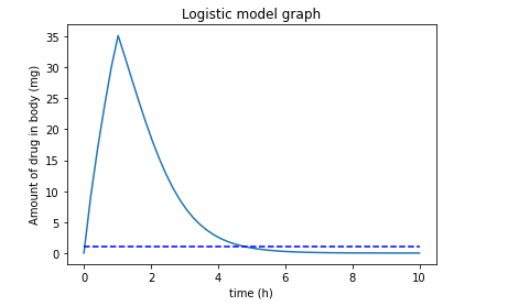
\includegraphics[scale = 0.7]{LogisticModelGraph.png}
\end{center}


Again the point $A(t) = k$ or when the amount of drugs in the body equals the new absorption parameter, there is a peak in the body and afterwards it will decay. As time goes on more drugs will be disposed which is different from the base model that decays exponentially.\\

For the Logistic model, when we do the derivative of $dA/dt$ and substitute the value the equilibria. If the value is greater than 0, then the equilibria is unstable. If the value is lower than 0, then the equilibria is stable.

The stability tells us when the maximum will occur which is crucial to know when we can expect when the drugs will be disposed so we can re dose to maintain concentration. Again, similar to the other models, the drug will be undetected after 4 hours. 



\subsection*{Analytical solution of Logistic Model}
When $0 \leq t \leq h$, the model equation is  $\frac{dA}{dt} =r-cA(1-\frac{A}{k})$.
$\frac{1}{r-cA(1-\frac{A}{k})}dA = dt$

Let $u = r-cA(1-\frac{A}{k})$\\
$$
dA = \frac{1}{-c+\frac{c}{k}A}du.\\
$$
$$
\frac{1}{u}( \frac{1}{-c+\frac{c}{k}A})du = dt
$$
$$
\int_{u(A(0))}^{u(A(t))} \frac{1}{u}( \frac{1}{-c+\frac{c}{k}A})du = \int_{0}^{t} dt\\
$$
$$
\frac{ln (u)}{-c+\frac{c}{k}A} = t + n
$$
put $u = r-cA(1-\frac{A}{k})$ back.
$$
ln(r-cA(1-\frac{A}{k})) = (-c+\frac{c}{k}A)t + n
$$

$$
r-cA(1-\frac{A}{k}) = e^{(-c+\frac{c}{k}A)t + n}
$$
The analytical solution of this model when $t \in [0,h]$ will be
$$
A(t) = \frac{k}{r + re^{-ct+n}}
$$
When $ t > h$, the model equation is  $\frac{dA}{dt} =-cA(1-\frac{A}{k})$.
$\frac{1}{-cA(1-\frac{A}{k})}dA = dt$

Let $u = -cA(1-\frac{A}{k})$\\
$$
dA = \frac{1}{-c+\frac{c}{k}A}du.\\
$$
$$
\frac{1}{u}( \frac{1}{-c+\frac{c}{k}A})du = dt
$$
$$
\int_{u(A(0))}^{u(A(t))} \frac{1}{u}( \frac{1}{-c+\frac{c}{k}A})du = \int_{0}^{t} dt\\
$$
$$
\frac{ln (u)}{-c+\frac{c}{k}A} = t + n
$$

put $u = -cA(1-\frac{A}{k})$ back.
The analytical solution of this model when $t \in [0,h]$ will be
$$
A(t) = \frac{-k}{1+ne^{-ct}}
$$
Connecting with the real world, the original model

$\frac{dA}{dt}=r-cA(1-\frac{A}{k})$ has one more factor which can affect the time to absorb the drug in the body. We assume k is times the blood can flow a round per hour. If $r$ and $c$ are constant, k increases, the time which the drug go through the body will shorter. This means the body will absorb the drug at a much faster rate. This can more accurately model those with faster processing rates due to their genetics or lifestyle habits which in then can be studied on how to maximize efficiency of drug. 

Overall, describing the processing rate as a logistic model, we see that between time 0 and h, and time past h, each have a stable and unstable equalibrium. Compared to the base model where all equilibrium are stable. The new absorption parameter K, changes how the drug increases in the body by being almost linear, still exponential compared to the base model which was parabolic. This means the change is constant and steady before it exponentially decays. In conclusion, people have different processing rates of the same drug and so different equations and parameters need to be introduced to accurately model them to ensure safety and reliability of drugs before they are administrated. 

\section*{Age related model}
We would like to explore how age affects how the vaccine is dosed and how the body processes the drug. Age is a huge factor when ensuring safety of a drug. For the COVID vaccine, children under the age of 5 were not given the vaccines initially because more tests and experiments needed to be done to make sure it was effective. Children have different processing rates and adults and seniors and understanding these differences will help scientists make sure it is safe for everyone to use. This extension is especially prevalent for drugs that treat diseases that usually children get such as chicken pox.\\
\\
By comparing people of different ages, we can conclude that compared with the adult from 18 to 40, the bodies of children and elders will metabolize drugs much worse. Since children's bodies are not yet fully developed, if the dose of the drug is too large, the drug will turn into a toxic substance in the body of the children. For elders, the poor ability of their bodies to metabolize drugs is mainly due to the gradual aging of the body. And in the research we know that under the oral method, one of the most organs for metabolism is liver. In the merck manuals it says Metabolism is also affected by aging, decreasing by about 1 percent per year after age 40 (merckmanual,2021). So if we assume k is the age. Then $k-40$ will be the years after 40. $c(1-0.01(k-40))$ will become $(1.4c-0.01ck)$ The metabolic function of the elderly is slightly better than that of children who are not fully developed. In general, Resting metabolic rate averaged 4.93 ± 1.09 for adults and 3.91 ± 0.98 for children (National library of medicine,2007). From the data point of view, adults do have a faster metabolic rate than children. When using the Pfizer vaccine, it is 3 to 5 micro-grams for children under 5 years old, and 30 micro-grams for adolescents and adults(cbc,2021).
\\
\\
Related to Age
\begin{equation}
  D(t) =
    \begin{cases}
      r & \text{if  $0 \leq t \leq h$}\\
      0 & \text{if $h< t$}
    \end{cases}       
\end{equation}

\begin{equation}
  P(A) =
    \begin{cases}
      cA(t) & \text{if  $0 \leq k \leq 40$}\\
      (1.4c-0.01ck)A(t) & \text{if $40 < k$}
    \end{cases}       
\end{equation}

In the model equation, all the elements are same as the basic model except one parameter K, representing age. From the research, notice that when the age ranges from 5 to 18, the ability of metabolism is continue to growing up to the level of adults, age 18 and staying at the same level until the age of 40. During this period, the clearance rate is linear. After the age of 40, the ability of metabolism will decrease as the age increase. During this period, the clearance rate is slowing down due to the age increasing.

\begin{equation}
  \frac{dA}{dt} =
    \begin{cases}
      5-cA(t) & \text{if  $k \leq 5$}\\
      30-cA(t) & \text{if $5 < k \leq 40 $}\\
      30- (1.4c-0.01ck)A(t) & \text{if $40 < k$}
    \end{cases}       
\end{equation}

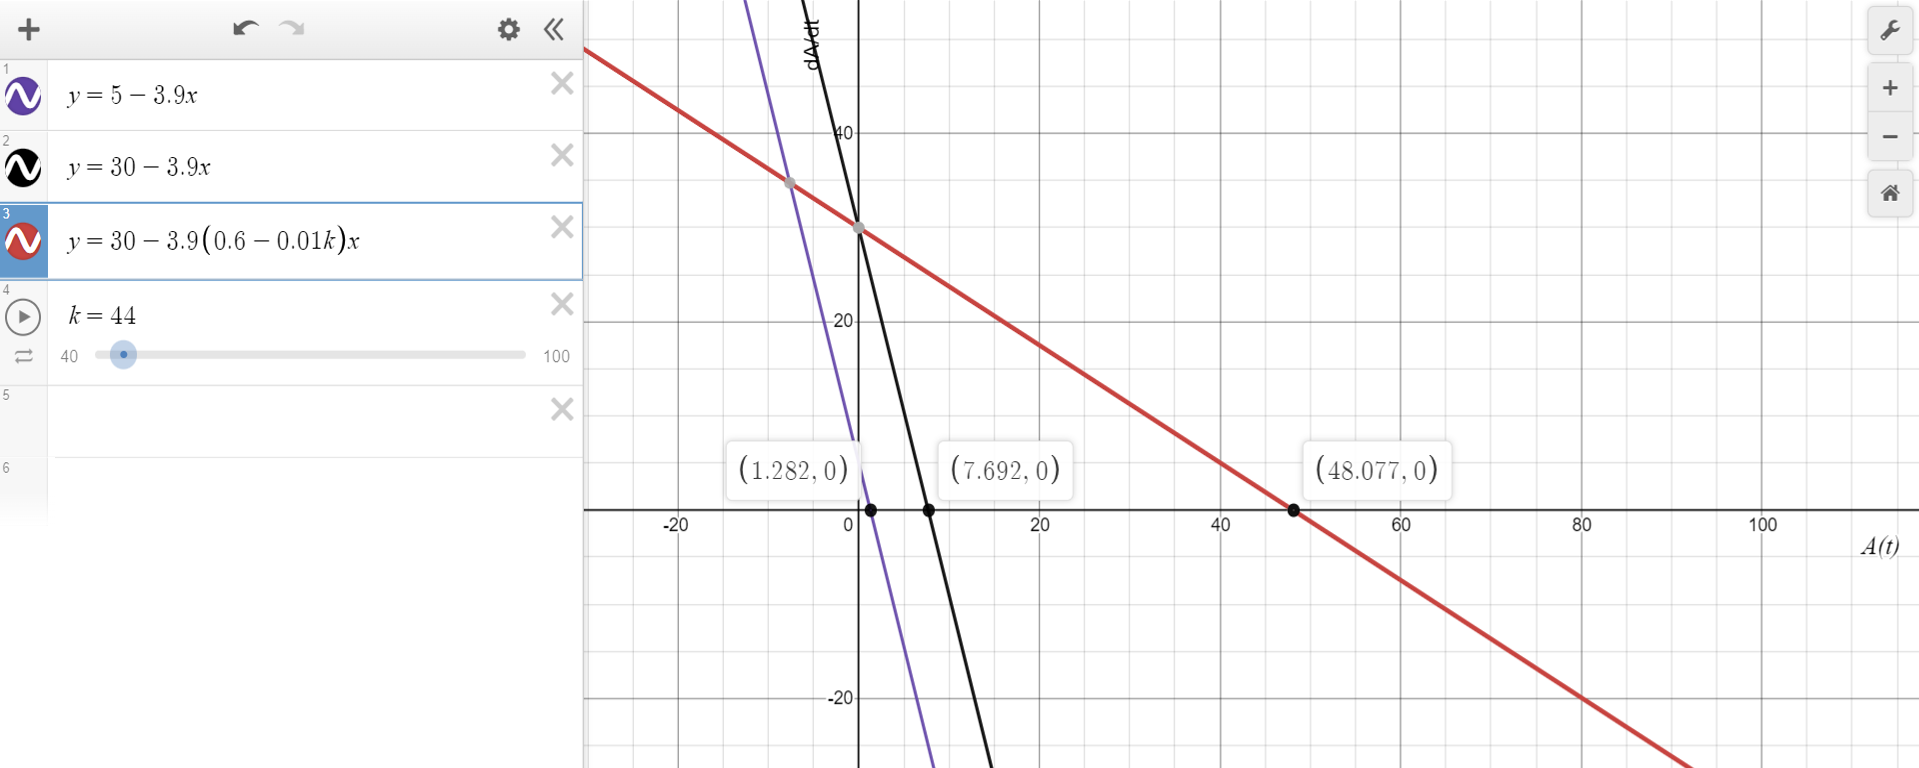
\includegraphics[scale = 0.4]{extension general graph.png}

For the blue line which is the graph of the changes of drugs in children's body. Since during  this time, children's body is still growing so their body will cost more energy which means their metabolism rate is even higher than the adults. Then the black line is dA/dt for the age from 5 to 40. During this period, the body will not need to spend as much as energy to metabolism. Which means until age 40, the speed of metabolism is constant. Since for age from 5 to 40, the dose amount is more than under 5 based on the dose which is given by Pfizer vaccine, so the time which more than under 5. For the red line, which is going to be dA/dt of age over 40. In the description of extension model related to age, it said the metabolism ability will decrease 1 percent per year. So, the slope of graph will be more horizontal as the age increase, which means for elderly metabolising drug will need more time to reach 0.

These cases are going to mdoel the Pfizer vaccine. According to to the above model we can look at two cases $0 \leq t \leq h$ and $t < h$.

When $0 \leq t \leq h$:
\begin{equation}
  \frac{dA}{dt} =
    \begin{cases}
      r-cA(t) & \text{if  $0 \leq k \leq 40$}\\
      r- (1.4c-0.01ck)A(t) & \text{if $k > 40$}
    \end{cases}       
\end{equation}

When $t > h$:
\begin{equation}
  \frac{dA}{dt} =
    \begin{cases}
      -cA(t) & \text{if  $0 \leq k \leq 40$}\\
      -(1.4c-0.01ck)A(t) & \text{if $k > 40$}
    \end{cases}       
\end{equation}

\section*{Age related extension analysis}
The first equation is same as the base model so the solution will also be the same. All we need to do is to use go through the same steps which are in base model analysis. 

\subsection*{Equilibria}
As the same as base model steps, to find equilibria we need to let $\frac{dA}{dt} = 0$. Then we can get $$r-cA(t)=0$$ and $$r-(1.4c-0.01ck)A(t)=0$$ We can get two respectively equilibria $A(t)=\frac{r}{c}$ and $A(t)=\frac{r}{1.4c-0.01ck}$. By the definition, r is the dose rate, c is the clearance rate and k is the age. Since c and k cannot be 0, so when $t>h$, r = 0, Another equilibria is A(t) = 0.\\
\\
\subsection*{Stability}
For $0 \leq t \leq h$, the stability will be the same as in the base model. The two equilibria $A(t)=\frac{r}{c}$ and $A(t)=\frac{r}{1.4c-0.01ck}$ are stable since the value around the equilibria moving towards to equilibria. In the graph,we assume that the age is 50. Then the pfizer vaccine dose rate is 30, let the clearance rate be 1.5, then the graph of $\frac{dA}{dt} =r-{c}A(t)$ and $\frac{dA}{dt} =r- (1.4c-0.01ck)A(t)$ will be the following.
\begin{center}
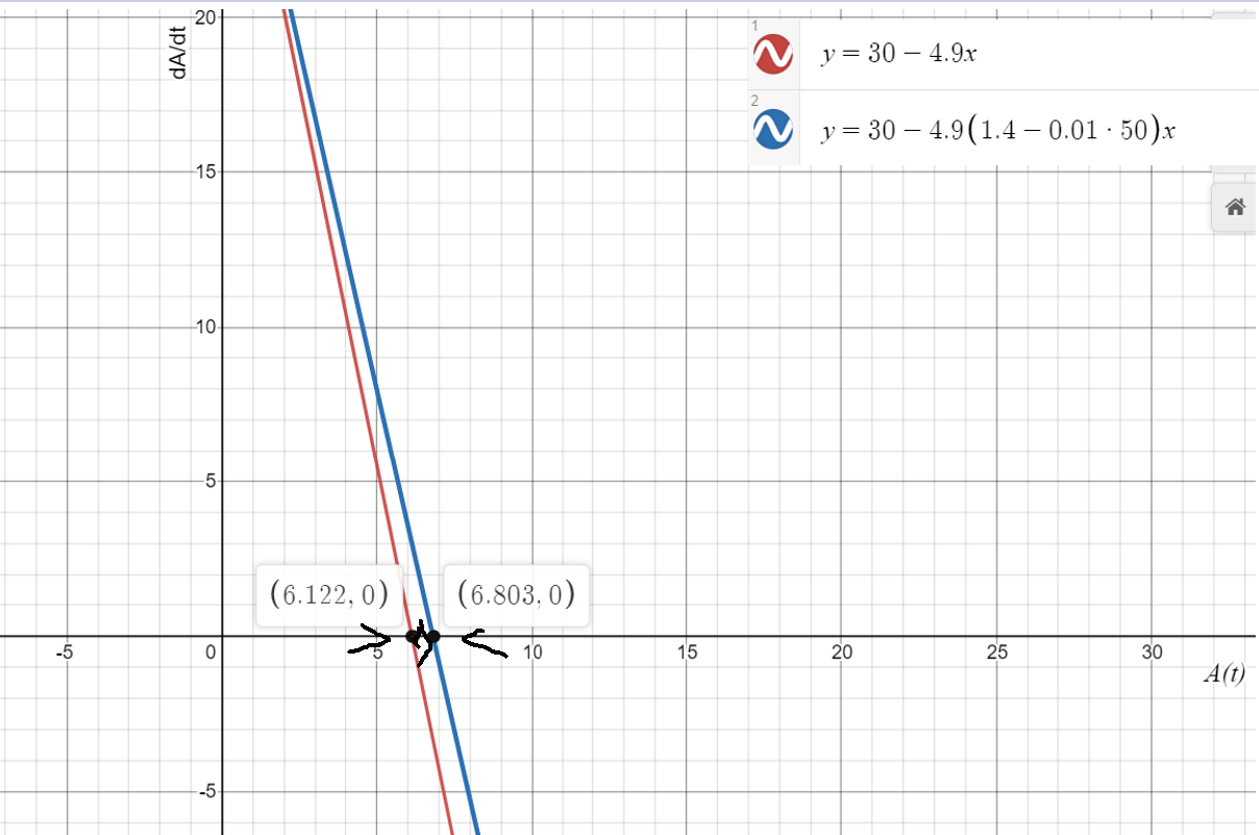
\includegraphics[scale = 0.43]{age graph 1.png}    
\end{center}


When $t > h$, the stability of the equilibria of $\frac{dA}{dt} =-{c}A(t)$ and $\frac{dA}{dt} =- (1.4c-0.01ck)A(t)$ will be stable.
\begin{center}
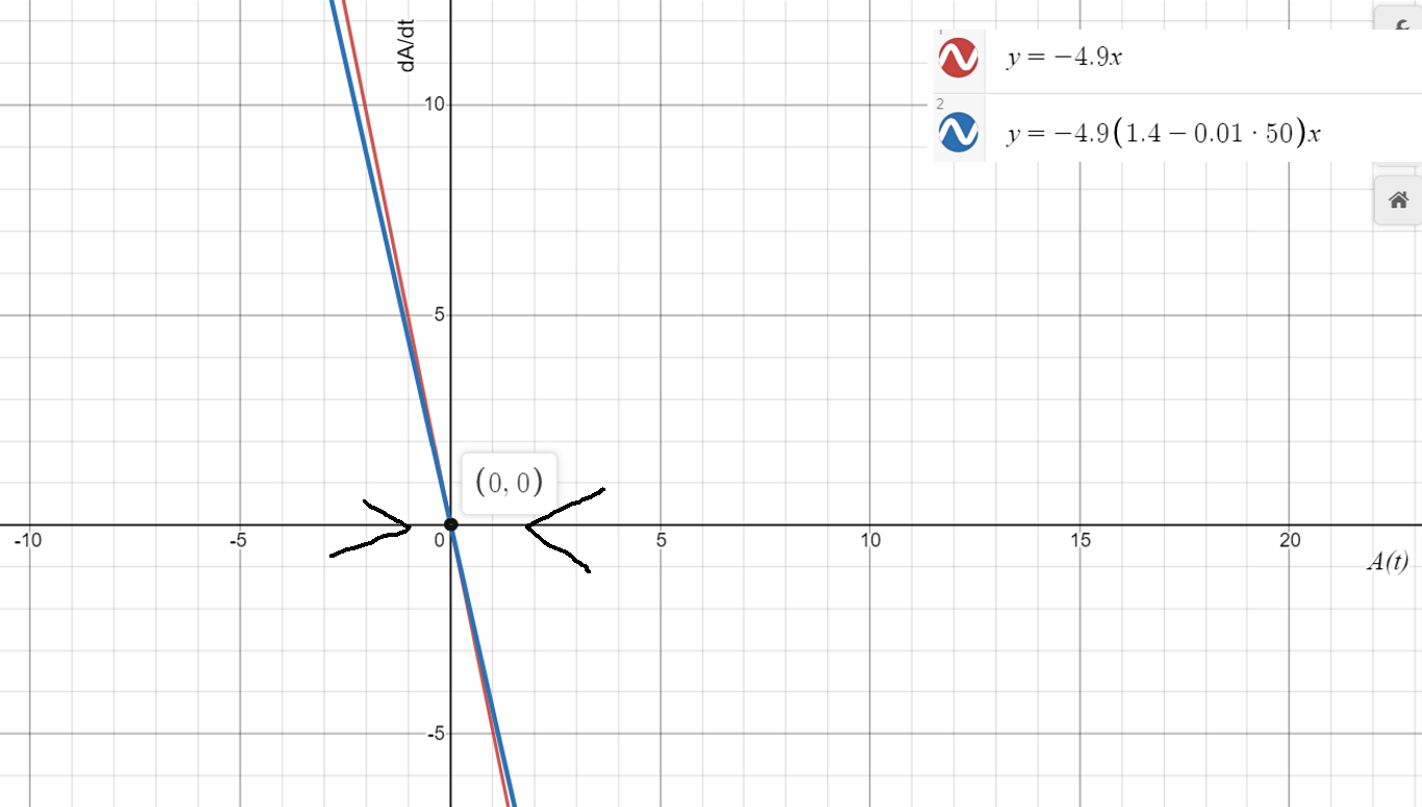
\includegraphics[scale = 0.43]{age graph 2.png}
    
\end{center}

\subsection*{Analytical solution}
When $0 \leq t \leq h$ and $k \leq 5$, the model equation is  $\frac{dA}{dt} =r-{c}A(t)$. When $t > h$ and $k \leq 5$, the model equation is $\frac{dA}{dt} =-{c}A(t)$. These two model equations have already be done in the base model analysis solution. For model equation $\frac{dA}{dt} =r-{c}A(t)$, The analysis solution is $A(t) = r(me^{-ct}-1)$ where m is a constant. And for model equation $\frac{dA}{dt} =-{c}A(t)$ is $A(t) = me^{-ct}$.\\
\\
When $0 \leq t \leq h$ and $k > 40$, the model equation is  $\frac{dA}{dt} =r-(1.4c-0.01ck)A(t)$.
$$
\frac{1}{r-(1.4c-0.01ck)A(t)}dA = dt
$$
Let $u = r-(1.4c-0.01ck)A(t)$. and $m = (1.4c-0.01ck) $\\
Then $u=r-mA(t)$, $dA = \frac{1}{0.01ck-1.4c}du$.\\
$$
\frac{1}{u}( \frac{1}{0.01ck-1.4c})du = dt
$$
$$
\frac{ln u}{0.01ck-1.4c} = t + n
$$
$$
\ln u(A(t)) - \ln u(A(0)) = (0.01ck-1.4c)t + n
$$
$$ln(u) = (t+n)(0.01ck-1.4c)$$

put u = r-(1.4c-0.01ck)A(t) back

The analytical solution is 
$$A(t) = \frac{-e^{(t+n)(0.01ck-1.4c)}+r}{(1.4c-0.01ck)}$$

From the two analytical solution of two model equations, we can can find that this is the inverse graph of exponential function. When we put the values to it, we can find that as the k increases, the drug in the body will need more time to become 0. This situation shows that as the ages increase the ability of metabolism will become worse which is fit to our research and the age will affect the body's metabolism of drug.

It is evident that people over the age of 40 have slower metabolism. The equilibrium are still stable so although the graphs are the same shapes, they are different due to different processing rates. Older people require more medications as they are growing weaker, so this information over people over the age of forty and comparing results can tell researchers a lot of what to keep in mind when creating medications. 

In conclusion, we can rely on these information to compare the behaviour of the drug between different age groups to create generalizations in order to further research effects of drugs. The finding of age increasing ability of metabolism is not a surprising factor, instead this can tell us that for children and seniors the drug will not be processed as efficiently and therefore prolonging the concentrations in the body. Different dosages need to be determined in order to counteract which can be studied further. 


\section*{Proposed Stochastic element}
Based on people's age, ethnicity, gender etc, they will have specific clearance rates that will affect the way the body processes the drug. People who exercises regularly, have a balanced diet, and living in comfortable conditions might have a higher clearance rate because their body is able to absorb the drug as perfectly desired. But this is not the case for every individual, they might have a condition or disease that prohibits their body to process the drug normally and these are situations to analyze to understand how the drug operates. 

In this part, the stochastic element for our base model will be the clearance rate. We are assuming the different clearance rate for different group of people such as gender, weight, age. Let's say we have 6 different people with clearance rate: 1.01, 1.02, 1.07, 1.05, 1.16, 1.20. This is based on the average clearance rate found in research in the base model analysis. So that we can calculate the standard deviation by $s = \sqrt{\frac{\Sigma (X-mean)^{2}}{n-1}}$, where s is the standard deviation, $\Sigma = sum \ of$, $X$ is each value, mean is the mean of the current value, $n$ is the number of value in the data set. After that we can get the mean value is 1.085, and standard deviation is $sd \approx 0.07765307$.\\

Then, we can use the data above to simulate the changing of amount of drugs by random clearance rate. By the python function, we simulated 100 times with different clearance rate. The data output is below.\\
\begin{center}
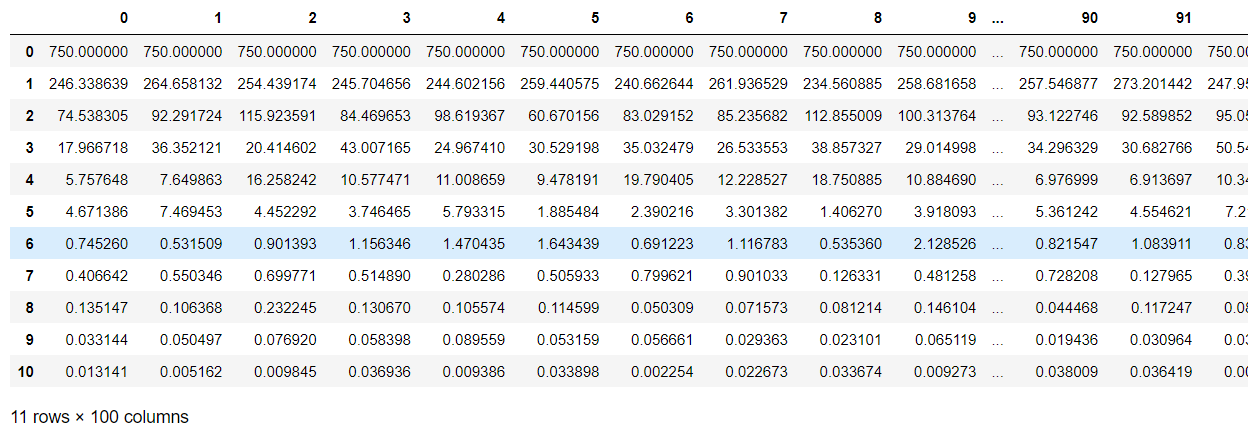
\includegraphics[scale = 0.47]{100Simulations.png}    
\end{center}
Combining with the data set above, we can plot the graph to see the distribution of of the stochastic simulation. Here, the graph at left is the distribution of 100 random clearance rate. Use that number, we can get the following distribution of amount of drugs after 5 hours. \\
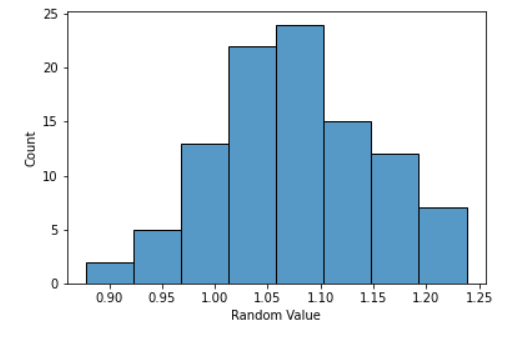
\includegraphics[scale = 0.5]{frequency distribution.png}
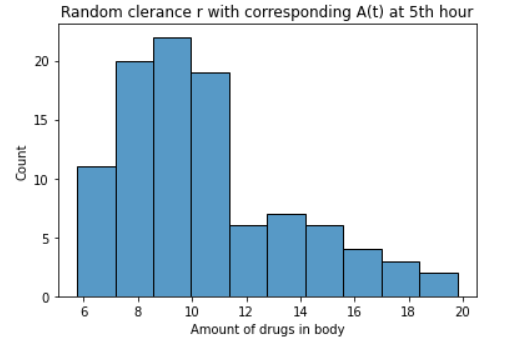
\includegraphics[scale = 0.5]{Distribution.png}


With a the same starting dosage of 750 milligrams, it is clear that when there are different clearance rates the time the body takes to process the drug is vastly dependent. With a mean clearance rate of 1.085 and standard deviation of 0.07765 we are able to see the how the amount in the drugs is affected by the clearance rate. If the clearance rate is below 1.085 the body will process it much slower compared to a clearance rate that is above 1.085. This is best described with the normal distribution with most people with a 1.05-1.1 unit per hour clearance rate. 

After doing 100 simulations we can see at hour 5 the distribution of people at each amount of drug. The people who have 6-10 milligrams have a faster clearance rate than those at 16-20 milligrams. This rightly skewed distribution will change as time goes on. So more people are in the below 10 milligrams because they are all processing it until it is undetected. This can also be used the other way around, looking at how much drug they have in their body at time t, we can calculate their clearance rate and be able to use this information for other research about the drug and understand it's abilities under different contexts and conditions. For example when we look at similarities of the group of people who have 18-20 milligram at hour five we can come to a conclusion that their similarity is the root cause of the processing rate. Then we can qualitatively measure the symptoms and affects on each individual and generally summarize which qualities of the body efficiently produce the best desired results. 


\section*{Discussion and Conclusion}

In review, our research question "How does the body process a drug that is administrated through oral methods comparatively to intravenous methods?"

Through mathematical calculations, stimulation's and analysis we can see there are advantages from oral medications and intravenous methods. Intravenous methods are much more effective because they are able to maintain a higher concentration for a longer period of time, but not all drugs desire this behaviour. Oral medications require less medical assistance in administration, medical waste, subject to error in dosing and is much more accessible and easy for the patient, yet it comes with its disadvantages of needed higher doses and the effects do not sustain as long. Intravenous methods on the other hand require less dosing and have longer effects but the medical waste of syringes are highly susceptible to infections and require medical professionals to administrate and monitor the patient for overdose and other allergic reactions. 

There is a clear difference in the rate of change of drugs in the body based on the delivery method. It is great to have different options for people's preferences of administration methods but looking a how the body will process the drug based on different elements such as age, gender, ethnicity, weight etc needs to be addressed when creating a drug. The two methods both have two stable equilibrium when the amount of drugs in the body are 0 and r/c. When the body processes the oral medication it will be a decaying exponential model and be undetectable after approximately 4 hours. 

For the intravenous method it is a graph that exponentially grows, reaches a peak like a parabola then follows the same decaying exponential model of disposing the drug as the oral method and becoming undetectable after approximately four hours.Each method is chosen based on accessibility and severity, for example a vaccine would typically be a shot because the effects and immunity would last months rather than a pill to resolve a headache is a quick remedy that effects will occur after a short period of time. 

These implications tell us how although both methods diminish at 4 hours, the behaviour in the body is drastically different. Furthermore, the stability of the equalibria shows when the predicted peak should be and therefore how the body should process the drug. In oral methods the peak is at time 0 and in the intravenous method the peak is at $t= \frac{r}{c}$ Both occur after dosing stops, but prolonging the peak will give longer lasting effects. 

Understanding the differences of how age factors how the body processes the body is vital. Children and seniors bodies will not process the same way a healthy adult does. They will require more assistance and different dosing rates. Their immunity or effects of the drug will be vastly different.

Some limitations in our models were having large ranges for each parameter. Some drugs can stay in the body for months and some for just a day. So when we want to model a general case it was difficult to generalize it to accurately represent a drug. Each drug is so specific in how to functions and each part of it is carefully constructed, so when creating our model we were finding different values for different drugs and trying to generalize it. When creating a drug all these factors of how, when and where the drug is administered are critical in producing the most efficient and desired effects and that is why these findings are crucial in the medical field. 

Moving forward, this project can explore other methods of administration such as intramuscular where the drug is injected into the muscle. More experiments and research can be collected in order to get more accurate simulations and equations. Other parameters need to be considered such as height, weight, eating and exercises habits as well as mental health. For example, marijuana would be an interesting study on different ages to see effects on the brain, IQ and physical and mental well being. As well, exploring what the models of the inefficient dose and overdose amount are vital to understand for safety measures. Mathematically, using a different base model where a elimination method could be considered for oral methods to account for how the drug is disposed before it even enters the bloodstream to get a more realistic result. These methods all have their advantages and disadvantages and depending on each drug, the model can describe the drugs desired behaviour in order to determine which is not only more effective more most accessible to the people who need it. 


\section*{Code}
Code for simulating oral medication.
\begin{center}
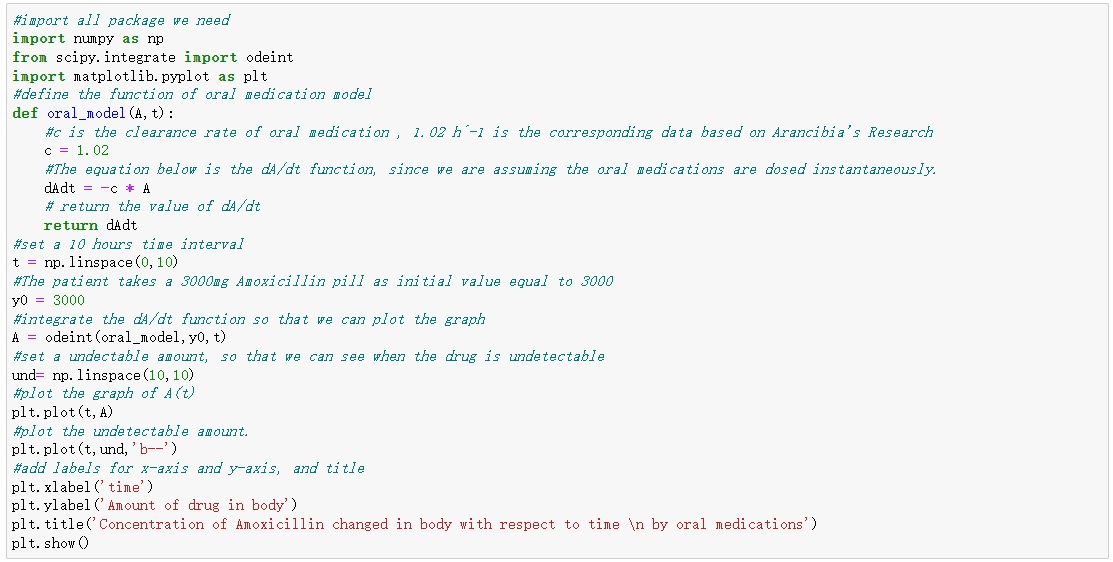
\includegraphics[scale = 0.6]{CodeOfOralSimulation.png} 
\end{center}
Code for simulating intravenous method.\\
\begin{center}
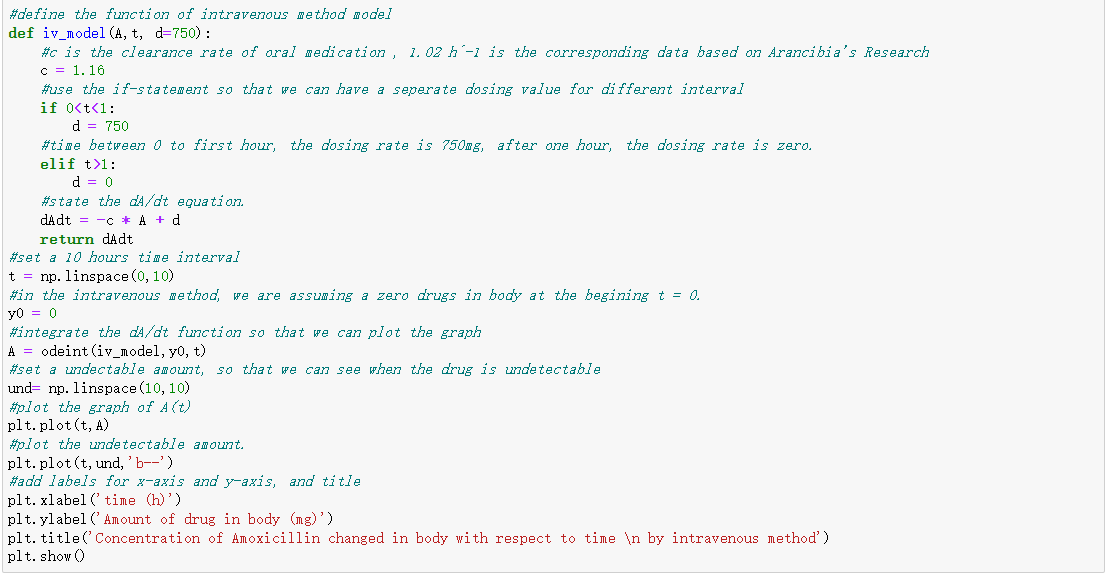
\includegraphics[scale = 0.6]{CodeOfIVSimulation.png} 
\end{center}
Code of Logistic model extension\\
\begin{center}
    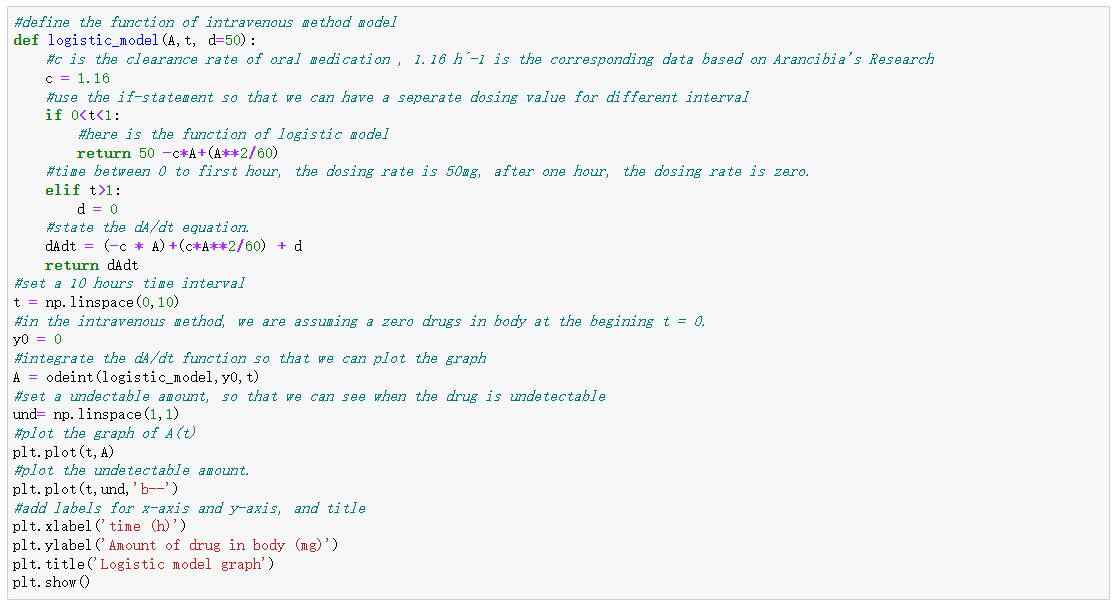
\includegraphics[scale = 0.6]{CodeOfLogistic.png}
\end{center}
Code of 100 times random simulation\\
\begin{center}
    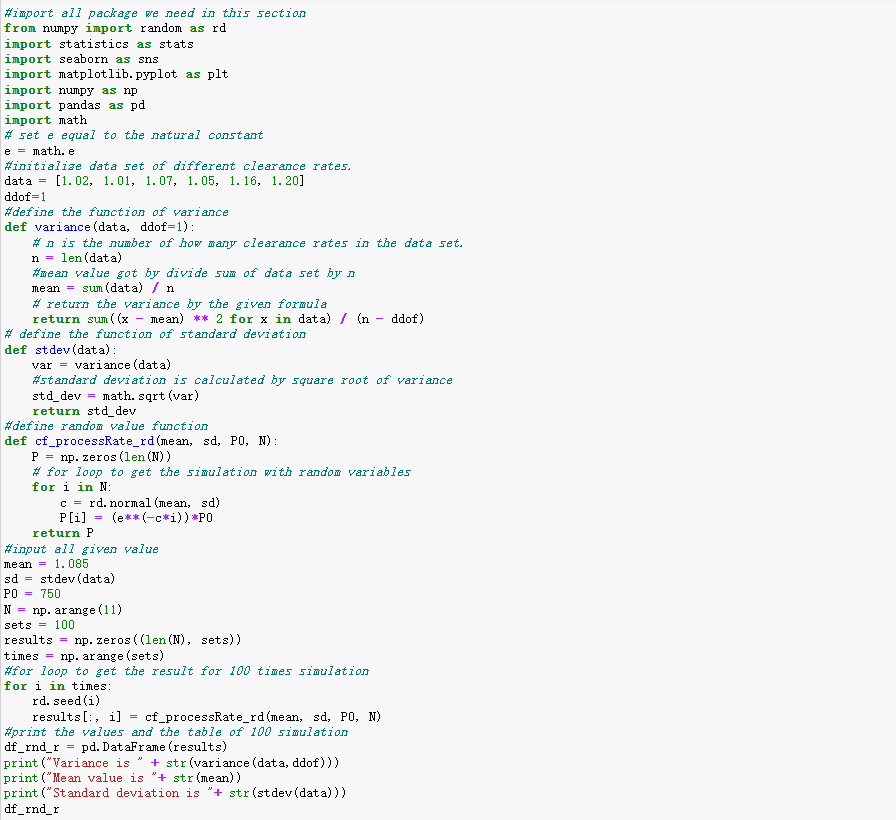
\includegraphics[scale = 0.65]{Codeof100simulation.png}
\end{center}
the corresponding output is\\
\begin{center}
    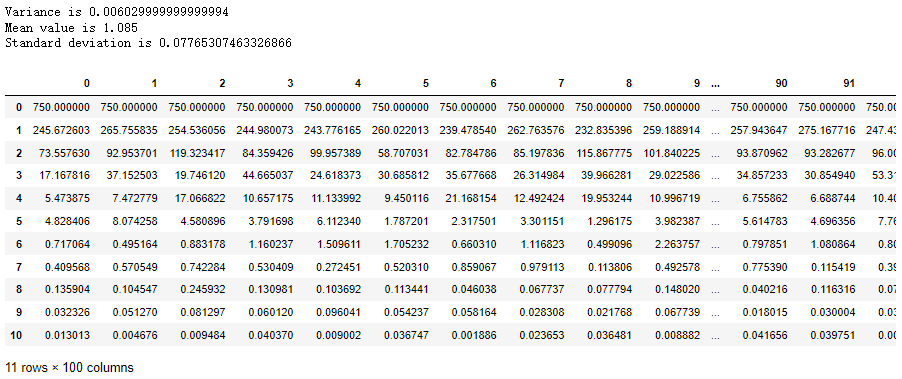
\includegraphics[scale = 0.6]{Corresponding out put of 100 simu.png}
\end{center}
Code of random clearance rate distribution\\
\begin{center}
    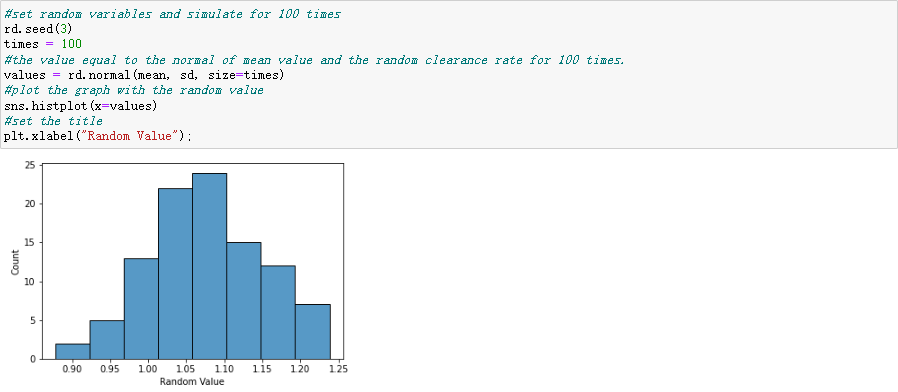
\includegraphics[scale = 0.6]{CodeOfRandomValue.png}
\end{center}
Code of amount of drug in body after 5 hours\\
\begin{center}
    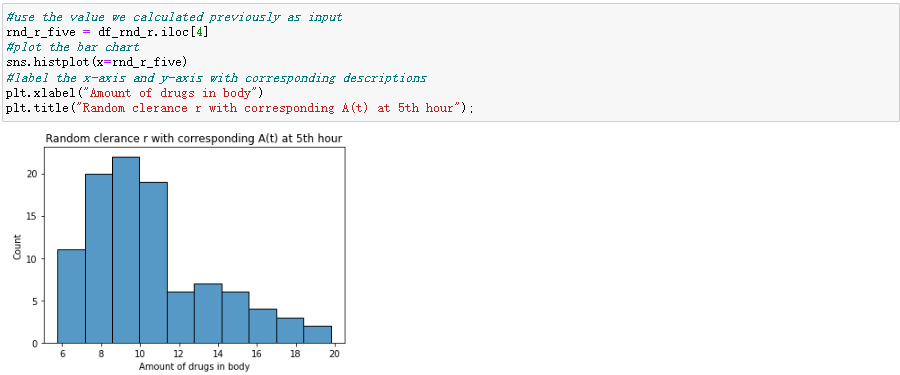
\includegraphics[scale = 0.6]{CodeOfdistribution_of_A(t).png}
\end{center}
\section*{Individual Contributions }

Gabriella researched all the statistics,wrote the base models, analyzed all the graphs, calculations, stability and related it to the real world context. She also wrote the discussion and conclusion,edited, and cited everything to ensure consistency. 

Junze calculated all the analytical solutions, coded and research data for all the graphs, stimulated and explained all the models and edited the entire report to ensure consistency. 

William wrote the background and motivation and research question. 

Raymond wrote the analysis and did research for the logistic model and age extension. 



\section*{Citations}

Mikulic, M. (2022, March 11). Covid-19 drugs in development by phase. Statista. Retrieved March 15, 2022, from https://www.statista.com/statistics/1119060/coronavirus-drugs-in-development-by-phase-worldwide/

Ritchie, H., Mathieu, E., Rodés-Guirao, L., Appel, C., Giattino, C., Ortiz-Ospina, E., Hasell, J., Macdonald, B., Beltekian, D., & Roser, M. (2020, March 5). Coronavirus (COVID-19) vaccinations. Our World in Data. Retrieved March 15, 2022, from https://ourworldindata.org/covid-vaccinations?country=OWIDWRL 

Reed, J., & Carmichael, G. (2022, March 16). Autocoding adverse events to meddra – time to throw out the manual... Linguamatics. Retrieved April 1, 2022, from https://www.linguamatics.com/solut\\ions/drug-development-safety-and-pharmacovigilance 

 Khanday, M. A., Rafiq, A., & Nazir, K. (2016, July 26). Mathematical models for drug diffusion through the compartments of blood and Tissue Medium. Alexandria Journal of Medicine. Retrieved March 15, 2022, from https://www.sciencedirect.com/science/article/pii/S2090506816300136 

R. Scott Obach, Nina Isoherranen, (2022) Chapter 10 - Pathways of drug metabolism, Editor(s): Shiew-Mei Huang, Juan J.L. Lertora, Paolo Vicini, Arthur J. Atkinson, Atkinson's Principles of Clinical Pharmacology (Fourth Edition), Academic Press, 2022, Pages 151-168, ISBN 9780128198698, https://doi.org/10.1016/B978-0-12-819869-8.00001-X.

Le, J. (2022, March 30). Drug metabolism - clinical pharmacology. Merck Manuals Professional Edition. Retrieved April 3, 2022, from https://www.merckmanuals.com/professional/clinical-pharmacology/pharmacokinetics/drug-metabolism 

Centers for Disease Control and Prevention. (n.d.). Pfizer-biontech COVID-19 vaccine overview and Safety. Centers for Disease Control and Prevention. Retrieved March 16, 2022, from\\ https://www.cdc.gov/coronavirus/2019-ncov/vaccines/different-vaccines/Pfizer-BioNTech.html 

Davis, N. (2021, August 12). Energy to burn: Teenage metabolism rate similar to adults', says study. The Guardian. Retrieved March 18, 2022, from \\https://www.theguardian.com/science/2021/aug/12/energy-to-burn-teenage-metabolism-rate-similar-to-adults-says-study#:~:text=%E2%80%9CIt%20seems%20to%20be%20a,constant%20access%20to%20the%20fridge. 

Ema. (2021, January 20). Extra dose from vials of Comirnaty COVID-19 vaccine. European Medicines Agency. Retrieved March 16, 2022, from https://www.ema.europa.eu/en/news/extra-dose-vials-comirnaty-covid-19-vaccine 

How does the body metabolize medication? Orlando Clinical Research Center. (2019, May 22). Retrieved March 30, 2022, from https://ocrc.net/how-does-the-body-metabolize-medication/#:~:text=In%20general%2C%20it%20typically%20takes,therapeutic%20to%20reach%20the%20bloodstream. 

How long do IV fluids stay in the body? HEALTH. (n.d.). Retrieved March 30, 2022, from https://www.next-health.com/blogs/news/how-long-do-iv-fluids-stay-in-body 

Le, J. (2022, March 17). Drug administration - drugs. Merck Manuals Consumer Version. Retrieved March 30, 2022, from https://www.merckmanuals.com/en-ca/home/drugs/administration-and-kinetics-of-drugs/drug-administration 

Khanday, M. A., Rafiq, A., & Nazir, K. (2016, July 26). Mathematical models for drug diffusion through the compartments of blood and Tissue Medium. Alexandria Journal of Medicine. Retrieved March 15, 2022, from https://www.sciencedirect.com/science/article/pii/S2090506816300136

Mayo Foundation for Medical Education and Research. (2022, March 1). Penicillin (oral route, injection route, intravenous route, intramuscular route) proper use. Mayo Clinic. Retrieved March 30, 2022, from https://www.mayoclinic.org/drugs-supplements/penicillin-oral-route-injection-route-intravenous-route-intramuscular-route/proper-use/drg-20062334 

Mikulic, M. (2022, March 11). Covid-19 drugs in development by phase. Statista. Retrieved March 15, 2022, from https://www.statista.com/statistics/1119060/coronavirus-drugs-in-development-by-phase-worldwide/

Ritchie, H., Mathieu, E., Rodés-Guirao, L., Appel, C., Giattino, C., Ortiz-Ospina, E., Hasell, J., Macdonald, B., Beltekian, D., & Roser, M. (2020, March 5). Coronavirus (COVID-19) vaccinations. Our World in Data. Retrieved March 15, 2022, from https://ourworldindata.org/covid-vaccinations?country=OWID_WRL

Vela Ramirez, J. E., Sharpe, L. A., &amp; Peppas, N. A. (2017, May 15). Current state and challenges in developing oral vaccines. Advanced drug delivery reviews. Retrieved March 30, 2022, from https://www.ncbi.nlm.nih.gov/pmc/articles/PMC6132247/ 

Wenderoth, B. (2022, January 31). What is IV therapy? what you should know. Mobile IV Medics. Retrieved March 30, 2022, from https://mobileivmedics.com/what-is-iv-therapy/#:~:text=The%20effects%20can%20last%20for,45%20minutes%20to%20an%20hour. 

Zhang, L., Wang, W., &amp; Wang, S. (2015). Effect of vaccine administration modality on immunogenicity and efficacy. Expert review of vaccines. Retrieved March 30, 2022, from https://www.ncb\\i.nlm.nih.gov/pmc/articles/PMC4915566/ 

EMC of European Medicines Agency. (2018, Jan 10). Amoxicillin Sodium for Injection, from https://www.medicines.org.uk/emc/product/1358/smpc#gref

EMC of European Medicines Agency. (2022, Feb 07) Amoxicillin 3g Sachet Sugar Free, from https://www.medicines.org.uk/emc/product/4003/smpc#POSOLOGY

A. ARANCIBIA, J. GUTTMANN, G. GONZALEZ, AND C. GONZALEZ2. (1980, February).Absorption and Disposition Kinetics of Amoxicillin in Normal Human Subjects. Vol.17, No.2,p.199-202, ANTIMICROBIAL AGENTS AND CHEMOTHERAPY, \\
from https://www.ncbi.nlm.nih.gov/pmc/articles/PMC283758/pdf/aac00382-0105.pdf

Fernandez, E., Perez, R., Hernandez, A., Tejada, P., Arteta, M., & Ramos, J. T. (2011). Factors and Mechanisms for Pharmacokinetic Differences between Pediatric Population and Adults. Pharmaceutics, 3(1), 53–72. https://doi.org/10.3390/pharmaceutics3010053

J. Mark Ruscin & Sunny A. Linnebur(Jul 2021), Pharmacokinetics in Older Adults, https://www.merck \\manuals.com /en-ca/professional/geriatrics/drug-therapy-in-older-adults/pharmacokinetics-in-older-adults#:~:text=First%2Dpass%20metabolism%20(metabolism%2C,have%20higher%20circulating%20drug%20concentrations.

David G. Le Couteur, Andrew J. McLachlan, Rafael de Cabo, Aging, Drugs, and Drug Metabolism, The Journals of Gerontology: Series A, Volume 67A, Issue 2, February 2012, Pages 137–139, https://doi.org/10.1093/gerona/glr084

CBC News(Feb 22 2022), What we know about COVID-19 vaccines for kids under 5, CBC, https://www.cbc.ca/radio/whitecoat/what-we-know-about-covid-19-vaccines-for-kids-under-5-1.\\6345326#:~:text=The%20Food%20and%20Drug%20Administration,be%20available%20in%20early%20April.

Jennifer Le. (Oct 2020), Drug Metabolism, Merck Manual. https://www.merckmanuals.com/en-ca/professional/clinical-pharmacology/pharmacokinetics/drug-metabolism#:~:text=Drugs%20can%20be%20metabolized%20by,more%20concentrated%20in%20the%20liver.

J Pharmacol Pharmacother.(Apr 2014), Switch over from intravenous to oral therapy: A concise overview. doi: 10.4103/0976-500X.130042 from https://www.ncbi.nlm.nih.gov/pmc/articles/PMC4008927/

Kostyak, J. C., Kris-Etherton, P., Bagshaw, D., DeLany, J. P., & Farrell, P. A. (2007). Relative fat oxidation is higher in children than adults. Nutrition journal, 6, 19. https://doi.org/10.1186/1475-2891-6-19
\end{document}


\end{document}
